%% =====================================================================
%% Cross-Border Reasoning-Token Market -- SIGKDD Datasets & Benchmarks Track
%% v1.0 TEXT EDITS (2026-11-10, Asia/Shanghai). Working copy of
%% docs/latex-sigkdd/ rewritten to docs/PROTOCOL_v1.0.md + group decisions.
%% Pass 6: 40-seller main table, Review-locked wording, A2, EXP3 appendix.
%% Pass 12: official v1.2 Decision A result 1; generated router x audit T1.
%% v1.0 baselines preserved; v1.2 sources: results/v1.1/v1.2_decision_a_eval/.
%% See CHANGES_v1.0.md (Pass 6). Do not edit docs/latex-sigkdd/ (v0.1 copy).
%%
%% Track switch: the SIGKDD D&B Track is SINGLE-BLIND -> author names stay.
%%   Submission (current):   \documentclass[sigconf,review]{acmart}
%%   Research-track / double-blind ONLY (NOT this track):
%%                           \documentclass[sigconf,anonymous,review]{acmart}
%%   Camera-ready (later):   \documentclass[sigconf]{acmart}
%% =====================================================================
\documentclass[sigconf,review]{acmart}

%% ---- Front-matter metadata (no invented year/city/DOI) --------------
%% TODO(venue): fill \acmConference dates/location, \acmYear, \acmDOI,
%%   \acmISBN and \setcopyright from the official KDD rights form
%%   once the submission cycle is fixed. Left generic on purpose.
\setcopyright{none}
\settopmatter{printacmref=false}
\renewcommand\footnotetextcopyrightpermission[1]{}
\acmConference[KDD D\&B]{ACM SIGKDD Conference on Knowledge Discovery and Data Mining, Datasets and Benchmarks Track}{TBD}{TBD}
\acmDOI{}
\acmISBN{}

%% ---- Packages -------------------------------------------------------
\usepackage{CJKutf8}      % only for the Chinese affiliation line
\usepackage{listings}
\usepackage{tabularx}
\usepackage{makecell}
\usepackage{placeins}
\usepackage{newunicodechar}
\usepackage{xurl}        % allow line breaks anywhere inside \code{} identifiers/paths
\setlength{\emergencystretch}{3em}

%% Inline code / identifiers / paths: breakable typewriter text.
\DeclareUrlCommand\code{\urlstyle{tt}}
\makeatletter
\g@addto@macro\UrlBreaks{\do\_\do\=\do\|\do\,}
\makeatother

%% Safety net for stray Unicode in copied text.
\newunicodechar{≈}{\ensuremath{\approx}}
\newunicodechar{→}{\ensuremath{\rightarrow}}
\newunicodechar{∈}{\ensuremath{\in}}
\newunicodechar{−}{\ensuremath{-}}
\newunicodechar{⋈}{\ensuremath{\bowtie}}
\newunicodechar{×}{\ensuremath{\times}}

\lstset{basicstyle=\ttfamily\footnotesize,breaklines=true,columns=fullflexible,
  frame=single,framerule=0.3pt,xleftmargin=2pt,xrightmargin=2pt,
  commentstyle=\itshape,language=bash,keepspaces=true}

\newcommand{\qstar}{q^\star}
\newcommand{\pistar}{\pi^\star}
%% Visible placeholder for every v1.0 result that is not yet available.
\newcommand{\TBD}[1]{\textcolor{red}{[TBD: #1]}}
\newcommand{\Emet}{\mathrm{E}}
\newcommand{\Qmet}{\mathrm{Q}}
%% Caption note required on every table/figure that uses the first v1.0 batch.
\newcommand{\vzeroonenote}{\textbf{First batch, v0.1 scale (3 sellers); not the 40-seller main table.}}
%% Compact mean [lo, hi] cell for filled result tables.
\newcommand{\cil}[3]{\makecell[c]{#1\\[-0.35pt]{\scriptsize [#2, #3]}}}

% Generated by scripts/pass12_decision_a_tables.py; do not edit.
\newcommand{\DecisionAExample}{$0.110\rightarrow 0.021$}
\newcommand{\DecisionAExpQRange}{$-0.003$ to $-0.009$}


\begin{document}

\title{A Compliance-Constrained Reasoning-Token Market Simulator and Benchmark for Procurement under Sparse Audit Feedback}

%% Single author per draft; no coauthors, emails, ORCID, or funding invented.
%% TODO(author): add ORCID / email only if the submission system requires it.
\author{Yanjie Fu}
\affiliation{%
  \institution{University of Macau}
  \country{Macau SAR, China}}
\affiliation{%
  \institution{\begin{CJK}{UTF8}{bsmi}橫琴澳門大學高等研究院\end{CJK}}
  \country{China}}
\renewcommand{\shortauthors}{Yanjie Fu}

\begin{abstract}
Cross-border procurement of LLM inference increasingly looks like a marketplace: buyers route tasks under jurisdiction constraints, sellers post prices and capacities, and quality---and fraud---are revealed only partially and late. Existing simulators either study exchange microstructure (limit-order books, high-frequency trading) or bandit-style routing under \emph{immediate} correctness labels. Neither couples \textbf{hard compliance filters}, \textbf{strategic seller fraud} (model swap, token theft, and selective downgrade on hard questions), \textbf{escrow / slash settlement}, and \textbf{sparse or delayed outcome labels} in one reproducible generator.

We release a \textbf{compliance-constrained reasoning-token market simulator}---not a CLOB---together with a five-file JSONL schema, one-click export scripts, a leakage-checked public feature view, and a benchmark protocol frozen before the 40-seller main table (post-batch clarifications in Appendix~\ref{app:amend}). The platform has five layers: admission/compliance, routing and portfolio procurement, escrow settlement, oversight audit, and feedback/audit trails. Evaluation is \textbf{two-dimensional}: buyer exposure $\Emet$ (\code{fraud_share}) and seller intent $\Qmet$ (strategic sellers' learned attack probability while listed). Policies are shown as points on an $(\Emet,\Qmet)$ Pareto plot with intervals; we do not declare a winner, and the joint objective $J$, cost, and quality are appendix columns. Protocol tasks cover fixed-rate audit deterrence (T1), degradation of bandit routers as labels become sparse (T2), equal-budget adaptive audit as an appendix efficiency check (T3), and seller risk ranking from buyer-observable features (T4). Baselines include faithful reimplementations of PILOT and StageRoute (with its stage MIP), fixed routers, and random, fixed-rate, and risk-adaptive audits. Results use at least 20 seeds, paired-by-seed bootstrap intervals, and Holm correction. At 40 sellers, both bandit routers' $\Emet$ rises significantly as labels vanish; StageRoute's $\Qmet$ is identifiable and rises as $\pi$ falls, while PILOT's $\Qmet$ does not rise relative to $\pi=1$ (and is lower only at $\pi=0$ and $0.02$); the v1.0 48-round audit arms sit at low $\Emet$ mainly by rarely trading with strategic sellers. In this simulator, under default parameters at 1000 rounds, audits lower $\Emet$ and $\Qmet$ for both PILOT and strongest under the pre-run egreedy/fictitious-play/EXP3 rule (Decision A result 1) (\S\ref{sec:t1}). Official T4 (D3) is not scorable; a PILOT, $\pi=1$ supplement is in \S\ref{sec:t4}.
We do not propose a new deterrence or routing method; the contribution is the generator, schema, and protocol.
\end{abstract}

%% TODO(CCS): generate the official CCS XML + \ccsdesc lines with
%%   https://dl.acm.org/ccs and paste here. Not invented on purpose.
% \begin{CCSXML} ... \end{CCSXML}
% \ccsdesc[500]{...}

\keywords{benchmark, LLM inference procurement, reasoning-token market, compliance, audit, strategic fraud, sparse feedback}

\maketitle

%% =====================================================================
\section{Introduction}
\label{sec:intro}

Deployed LLM APIs are increasingly bought and sold across jurisdictions. A buyer in one country may be barred from shipping personal data to another; a seller may advertise a strong model and serve a weaker one (swap), serve the weaker one only on hard questions (selective downgrade), or bill for more reasoning tokens than were generated (theft); correctness labels for purchased answers arrive sparsely and often with delay. Procurement therefore mixes \textbf{compliance}, \textbf{strategic incentives}, and \textbf{incomplete feedback}---yet public benchmarks for this setting are scarce.

Two nearby literatures miss the coupling. Market-microstructure and exchange simulators emphasize continuous limit-order books, latency races, and circuit breakers---machinery that is orthogonal to posted-price reasoning services. Bandit and portfolio routers such as PILOT and StageRoute assume (or are evaluated under) rich, often immediate, outcome feedback and typically ignore strategic sellers and escrowed payments. Cloud-API SLA dispute stories and advertising-quality audits share the \emph{economic} idea of sampling and penalties, but do not ship a joinable, seed-locked generator for multi-jurisdiction reasoning procurement.

\textbf{This paper} treats the research artifact as a \textbf{platform that generates benchmarks}. We ask: can one simulator expose a stable evaluation surface for (i) deterrence under fixed audit budgets, (ii) sparse/delayed labels, (iii) audit-cost efficiency, and (iv) detecting risky sellers from what a buyer can actually observe---without claiming a new ``best router'' or ``best auditor''?

\paragraph{Contributions.}
\begin{enumerate}
\item \textbf{Five-layer trading platform} for compliance-constrained reasoning-service trades: admission $\rightarrow$ routing/portfolio procurement $\rightarrow$ escrow settlement $\rightarrow$ oversight $\rightarrow$ feedback and trails. Design principle: borrow \emph{audit economics} (sampling, slash, freeze); do \textbf{not} port CLOB, HFT, circuit breakers, or multi-CCP clearing.
\item \textbf{Publishable five-file JSONL schema} (\code{sellers}, \code{buyers}, \code{orders}, \code{audits}, \code{episodes}) with join keys and config hashes, a leakage-checked public feature view, and held-out label files; one-click scripts; a self-contained release pack (code MIT, data CC BY 4.0).
\item \textbf{Tasks T1--T4} under a protocol frozen before the 40-seller main table: a two-dimensional primary evaluation $(\Emet,\Qmet)$ reported as a Pareto plot without a declared winner; in this simulator, under default parameters at 1000 rounds, T1 finds lower $\Emet$ and $\Qmet$ for PILOT and strongest by the pre-run egreedy/fictitious-play/EXP3 rule (result 1); T2 reports sparse-label changes; T4 ranks sellers by future fraud risk from a fixed buyer-observable feature whitelist.
\item \textbf{Baselines}: faithful PILOT and StageRoute (with stage MIP), cheapest/strongest fixed routers, random-intensity audit ($a_t\sim U(0,2a)$ with $a=0.1$), fixed-rate audits $a\in\{0.05,0.1,0.2\}$ (the $a=0.1$ arm is the D3 reference baseline, not our method), and risk-adaptive audit; for T4, logistic regression, GBDT, and a rule.
\end{enumerate}

\paragraph{Scope.} This paper contributes the generator, the evaluation protocol, and the leaderboard contract; it does not propose or claim a new deterrence, routing, or detection method, and deterrence theory is out of scope.

%% =====================================================================
\section{Related Work}
\label{sec:related}

We situate the artifact against five nearby literatures. The gap we target is the \emph{coupling} of hard compliance filters, strategic seller fraud, sparse/delayed correctness labels, and escrow/audit settlement in one seed-locked generator---not incremental gains on any single line of work under dense feedback.

\paragraph{Cloud / API marketplaces and SLA disputes.} Commercial LLM/API marketplaces and cloud SLAs document uptime credits, refunds, and support-case dispute flows (e.g., provider compute SLAs and marketplace terms~\cite{aws2024compute_sla}), but they do not release multi-agent, seed-locked synthetic trade logs with jurisdiction hard filters and controllable strategic fraud knobs. Our contribution is a research generator and leaderboard contract, not a commercial marketplace replica.

\paragraph{Audit economics, inspection games, and advertising-quality sampling.} Classical enforcement and audit theory treat random inspection plus penalties as a deterrent when full verification is costly~\cite{becker1968crime,avenhaus2002inspection}. Advertising and product-quality settings similarly motivate sampling audits, reputation holds, and disclosure costs rather than exhaustive checks~\cite{daughety2008communicating,bester2021signaling}. We borrow \emph{sampling rate}, \emph{slash/penalty}, and optional \emph{freeze/delist}; we do \textbf{not} model ad auctions, click fraud scoring, or truth-in-advertising litigation.

\paragraph{Prediction-market dispute resolution and delayed labels.} Prediction markets separate trading from outcome resolution: optimistic oracles and dispute bonds (e.g., UMA-style resolution used by Polymarket) delay settlement until a challenge window closes or a vote completes~\cite{wolfers2004prediction,hanson2003combinatorial,uma2024optimistic,polymarket2024resolution}. That is a useful \emph{label-timing} analogy. In our platform the label channel $(\pi, L)$ is orthogonal to payment escrow: billed cost is observed immediately on the buyer side, while correctness may be delayed or dropped; audits update trust/slash on their own clock.

\paragraph{Bandit / portfolio LLM routing under immediate feedback.} PILOT~\cite{panda2025pilot} casts budgeted LLM routing as a preference-prior contextual bandit (LinUCB + online multi-choice knapsack). StageRoute~\cite{li2026stageroute} couples stage-wise deployment (a mixed-integer program over the deployed model set) with per-query budget/throughput LPs and near-optimal $\tilde{\mathcal{O}}(T^{2/3})$ regret. v1.0 ships \textbf{faithful reimplementations} of both, including StageRoute's stage MIP, each with unit tests against the original settings; we report either reproduction of the published numbers or the gap (\TBD{Coding: PILOT/StageRoute reproduction gap}). Both are designed for dense correctness labels; T2 measures how they behave when labels become sparse, which is a property of the setting, not a criticism of the methods.

\paragraph{Exchange surveillance vs.\ order-book microstructure.} Market-surveillance practice and guidance emphasize monitoring, investigation, and temporary freezes on suspicious activity~\cite{iosco2009surveillance,cumming2008surveillance}. Escrow, stake slash, and post-catch listing pauses in our oversight layer are inspired by that \emph{enforcement} toolkit. Continuous limit-order books, maker--taker fees, HFT latency races, and circuit breakers are explicitly \textbf{out of scope}---the market is posted-price routing / portfolio procurement, not a CLOB.

\paragraph{Positioning.} This paper covers the platform-as-benchmark-generator, five-file schema, Feature/Label hygiene, and the T1--T4 leaderboard contract. Whether fixed-rate audits change the strategic sellers' $\Qmet$ is posed as an empirical protocol question (T1, \S\ref{sec:protocol}), measured with the same metrics as every other arm; we claim no methodological novelty for audit design.

%% =====================================================================
\section{Platform Design}
\label{sec:platform}

The artifact is a \textbf{posted-price reasoning-service market} with jurisdiction-aware buyers and sellers. Buyers spend budget on tasks with gold answers; sellers advertise models, prices, and capacity. Matching is \textbf{routing / portfolio procurement}, not a limit-order book.

\subsection{Five layers (Figure~\ref{fig:layers})}
\label{sec:layers}

\begin{table}[t]
\caption{Five platform layers and their roles (code map in Appendix~\ref{app:repro}).}
\label{tab:layers}
\small
\begin{tabularx}{\columnwidth}{@{}>{\raggedright\arraybackslash}p{2.6cm} X@{}}
\toprule
Layer & Role \\
\midrule
1. Admission / compliance & Hard jurisdiction filters; blocked flows never become served purchases \\
2. Routing / portfolio procurement & Policy plugins (PILOT, StageRoute, fixed routers, audited cascades, \ldots) \\
3. Escrow settlement & State machine \code{locked} $\rightarrow$ \code{delivered} $\rightarrow$ \code{audited?} $\rightarrow$ \code{settled/slashed} (default \textbf{off}) \\
4. Oversight & Random, fixed-rate, or risk-adaptive audit; optional delist \\
5. Feedback \& trails & Label channel $(\pi, L)$ orthogonal to payment; structured audit fields \\
\bottomrule
\end{tabularx}
\end{table}

\paragraph{External surface.} Place order; delivery receipt; audit verdict; settlement; trail query (via joinable \code{orders}/\code{audits} exports).

\begin{figure}[t]
  \centering
  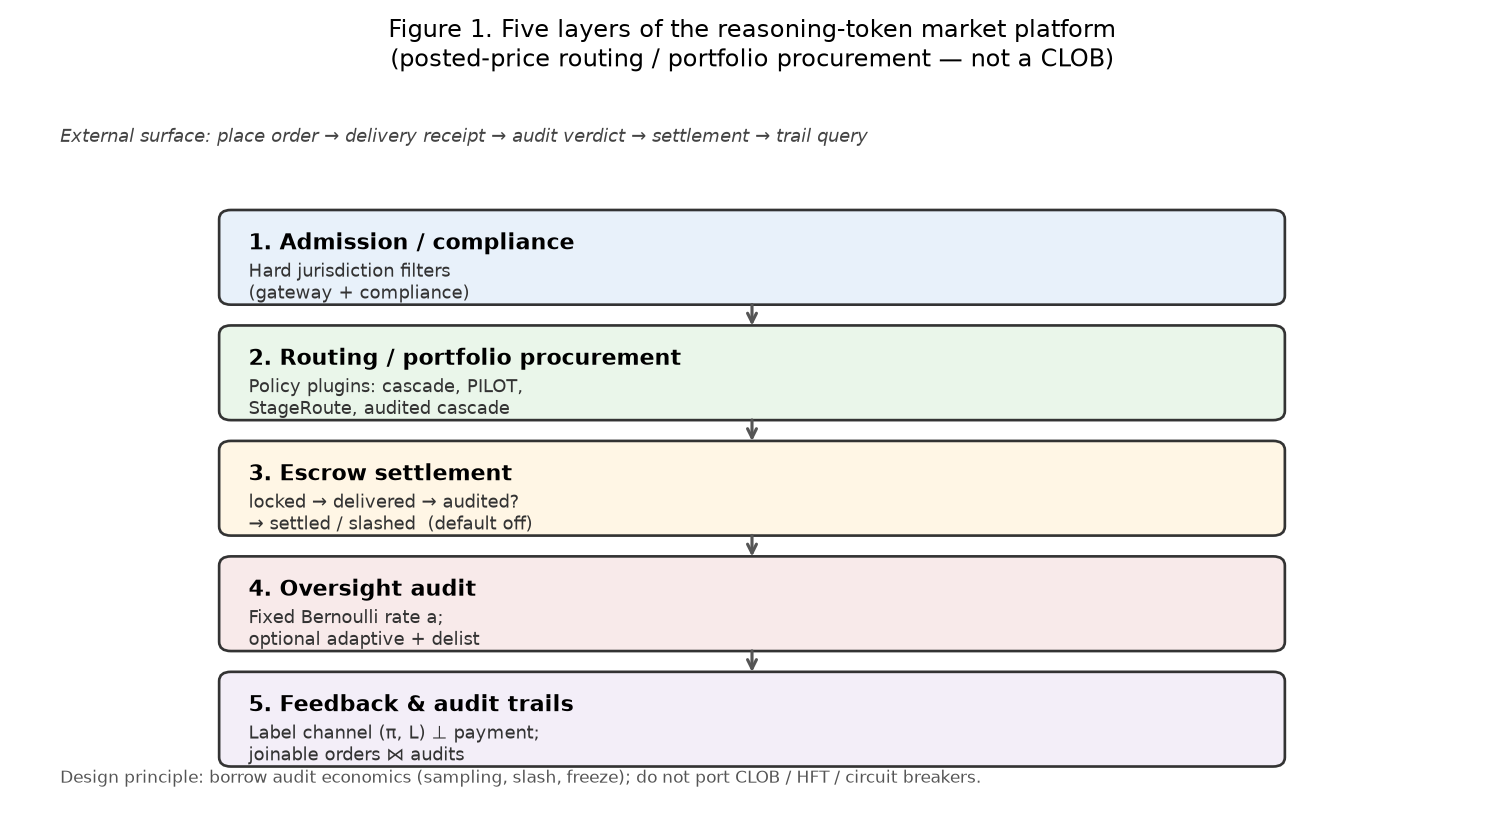
\includegraphics[width=\linewidth]{figures/fig1_five_layers.png}
  \caption{Five platform layers (admission $\rightarrow$ routing/portfolio procurement $\rightarrow$ escrow $\rightarrow$ oversight $\rightarrow$ feedback/trails). Posted-price market; not a CLOB.}
  \Description{Block diagram of the five platform layers of the reasoning-token market: admission and compliance, routing and portfolio procurement, escrow settlement, oversight, and feedback and trails.}
  \label{fig:layers}
\end{figure}

\subsection{Market primitives}
\label{sec:primitives}

\paragraph{Jurisdictions.} Synthetic CN / SG / BR corridors. Compliance profiles list allowed seller jurisdictions, sensitivity mixes, and consent rates. Rules are \emph{simplified simulations}---not legal advice (see Ethics).

\paragraph{Sellers.} Posted \code{list_price} (USD / 1k tokens), capacity per round, stake pool for slash. Headline configurations use 40 sellers (31 honest and 9 strategic: 3 swap / 3 theft / 3 downgrade). Calibration of list prices to public API price lists is \TBD{Coding: price sources, snapshot date, and mapping}; the present tables use the simulator's existing price ratios, not a public-list calibration. Strategic sellers learn attack probabilities for three attack types: \textbf{swap} serves a weaker \code{actual_model} than \code{claimed_model}; \textbf{theft} bills more reasoning tokens than were generated; \textbf{selective downgrade} swaps to a cheaper model only on hard questions.

\paragraph{Buyers.} Per-buyer budgets and strategy ids. Portfolio policies may purchase from multiple sellers per task under budget.

\paragraph{Audits.} A sampled audit runs identity and length checks with detection probabilities $d_{\mathrm{identity}}=d_{\mathrm{length}}=0.9$ and penalty $P=0.25$ in headline configs. Audits update slash / optional delist \textbf{immediately} (trust updates are disabled in Decision A by \code{trust_feedback=false}) and do not consume the correctness label channel.

\paragraph{Escrow (optional).} When enabled, seller proceeds are held until the audit decision; slash is taken from the hold. Escrow is \textbf{orthogonal} to label delay $L$.

\paragraph{Delist (optional).} After a catch, \code{reputation_rounds} suspends the seller from routing until a watermark round. Default \code{reputation_rounds=0}.

\subsection{Design principles}
\label{sec:principles}

Borrow: sampling audits, stake slash, payment freeze, structured trails.\\
Do \textbf{not} build: CLOB, price--time priority matching, HFT makers, circuit breakers, multi-CCP. Multi-buyer congestion is deferred to Limitations.

\subsection{Evaluation metrics}
\label{sec:metrics}

\paragraph{Buyer exposure $\Emet$.} $\Emet=$ \code{fraud_share} $=$ attacked served purchases / served purchases, where a purchase is attacked if it was swapped, token-stolen, or selectively downgraded (this is the formula in the simulator's metrics code; lower is better). $\Emet$ measures attacks that \emph{reach buyers}. The v0.1 column \code{active_attack_rate} used the same formula and is dropped. A billed-token-weighted variant $\Emet_{\mathrm{tok}}$ is a secondary side column in the v1.0 baseline Table~\ref{tab:t1-v10} and in Appendix~\ref{app:secondary}.

\paragraph{Seller intent $\Qmet$.} For each strategic seller, the attack probability $q$ it plays in each round, averaged \textbf{without weighting} over the last quarter of rounds (12 of 48 in v1.0; 250 of 1000 in Decision A) and \textbf{only over rounds in which the seller is listed}. Suspended rounds would otherwise move learned $q$ through missing observations, so the number of suspended rounds and the $q$ during suspension are reported separately and excluded from $\Qmet$. Per-mode columns $q_{\mathrm{swap}}$, $q_{\mathrm{theft}}$, $q_{\mathrm{downgrade}}$ are listed separately; the primary $\Qmet$ is their simple average (no token weighting). $\Qmet$ measures \emph{attack intent}, not attacks that reach buyers (lower is better).

\paragraph{Identifiability of $\Qmet$.} When a router avoids a seller so that it has no trades in the last quarter, attacking and not attacking pay the same and its $q$ is not driven by feedback. Tables report the \textbf{fraction of runs with tail-segment trades} ($\ge$1 strategic-seller trade in the last quarter) per policy and $\pi$; cells where most runs have no tail trades are drawn as hollow points and their $\Qmet$ receives no deterrence interpretation.

\paragraph{Pareto reading, no winner.} Each policy is one $(\Emet,\Qmet)$ point with 95\% interval bars on identifiable $\Qmet$. The text does not rank policies, declare a Pareto-front winner, or treat front membership from point estimates as a finding.

\paragraph{v1.0 gate for $\Qmet$ as a primary axis.} $\Qmet$ depends on how sellers learn. It stays a primary axis only if, at the 40-seller scale with the full baselines and \emph{at every} $\pi$, rerunning with fictitious play (the formal alternative) keeps the ordering of policies by $\Qmet$ (Kendall $\tau\ge 0.6$) \emph{and}, for points where $\Qmet$ is identifiable, the Pareto-front membership unchanged; otherwise $\Qmet$ is demoted to a side column and only $\Emet$ is primary. The pre-run mechanical rule passes: 8 identifiable methods under both egreedy and fictitious play, at every $\pi$, Kendall $\tau_a=0.643$ (23 concordant pairs, 5 discordant), just over 0.6, so $\Qmet$ remains primary. We do not call this ordering stable. Front membership in the gate computation is a point-estimate artifact and is not reported as a finding. A Hedge check on the first batch and an EXP3 check at 40 sellers are in Appendix~\ref{app:secondary}; neither counts toward this v1.0 gate. Decision A instead uses the pre-run multi-learner direction rule in \S\ref{sec:protocol}.

\paragraph{Secondary (appendix).} The joint objective
\begin{equation}
J = \mathrm{accuracy} - \lambda \cdot \mathrm{violation\_rate} - \mu \cdot \Emet,
\end{equation}
with $\lambda=1.0$, $\mu=0.5$, plus cost and quality, appear only in Appendix~\ref{app:secondary}. Accuracy is task-level (portfolio answer vs gold); violation rate is compliance breaches per task.

%% =====================================================================
\section{Data Release}
\label{sec:data}

\subsection{Five JSONL files}
\label{sec:files}

The v1.0 production boards in \code{release/v1.0/} are the reference release (schema dictionary and samples: Appendix~\ref{app:repro}). Small-scale pipeline-test exports are for pipeline testing only.

\begin{table}[t]
\caption{The five JSONL files.}
\label{tab:files}
\small
\begin{tabularx}{\columnwidth}{@{}l X@{}}
\toprule
File & Role \\
\midrule
\code{sellers.jsonl} & Catalog: jurisdiction, claimed model, listed quality, stake, ban watermark (labels held out) \\
\code{buyers.jsonl} & Budget, strategy\_id, compliance\_profile \\
\code{orders.jsonl} & State-machine fact table; join key \code{order_id} \\
\code{audits.jsonl} & Per served purchase: sampled checks, slash, delist, $\pi$/$L$ reveal fields (labels held out) \\
\code{episodes.jsonl} & Board --- one row per \code{(run_id, seed)}: $\Emet$, $\Qmet$, per-mode $q$, suspended rounds \\
\bottomrule
\end{tabularx}
\end{table}

\paragraph{Sample fields.} Table~\ref{tab:samples} shows compact sample keys; full dictionaries and three-row samples are in the schema documentation (Appendix~\ref{app:repro}).

\begin{table*}[t]
\caption{Sample fields (truncated; no secrets). Rows are schema illustrations; v1.0 values come from the v1.0 production export.}
\label{tab:samples}
\small
\begin{tabularx}{\textwidth}{@{}l X@{}}
\toprule
File & Compact sample keys $\rightarrow$ values \\
\midrule
\code{sellers} & \code{seller_id=seller_cn}, \code{jurisdiction=CN}, \code{claimed_model=Qwen/Qwen2.5-1.5B-Instruct}, \code{list_price}=\TBD{Coding: calibrated price}, \code{listed_quality}, \code{seed=0} \\
\code{buyers} & \code{buyer_id=buyer_cn_1}, \code{jurisdiction=CN}, \code{budget_total}, \code{strategy_id}, \code{seed=0} \\
\code{orders} & \code{order_id=}\ldots\code{|t0000_p059|0|seller_br}, \code{state=settled}, \code{tokens_billed}, \code{latency_ms}, \code{attack_mode} \emph{(held-out label)} \\
\code{audits} & \code{sampled}, \code{reveal_pi}, \code{label_delay_L}; \code{hit}, \code{slash_amount}, \code{fraud_realized} \emph{(held-out labels)} \\
\code{episodes} & \code{a}, \code{pi}, \code{fraud_share} ($\Emet$), $\Qmet$ and per-mode $q$, suspended rounds, \code{J} \emph{(appendix)}, \code{config_hash}=\TBD{Coding: v1.0 hash; final field names} \\
\bottomrule
\end{tabularx}
\end{table*}

\paragraph{Join keys.} \code{run_id}, \code{seed}, \code{order_id} (= \code{purchase_id} when served), \code{config_hash} (sha256 prefix of config).

\paragraph{Derived (not shipped).} Ledger / full event timeline = \code{orders} $\bowtie$ \code{audits}.

\subsection{Feature / Label separation}
\label{sec:featlabel}

Several fields are \textbf{evaluation labels}, not public training features; a model that uses them as inputs \textbf{leaks} the supervision signal. v1.0 strips the blacklist (Table~\ref{tab:labels}) from the public feature view before release; an export-time leakage check rejects any column outside the whitelist, including derived differences such as \code{tokens_actual}$-$\code{tokens_billed}. For T4, labels of the training runs are public, and labels of the test runs are withheld and scored only by the evaluation script.

\paragraph{How to submit.} A T4 entry is a file with one risk score per (test run, seller); the evaluation script computes the metrics of \S\ref{sec:t4protocol} against the withheld labels (script path and submission channel: \TBD{Coding: T4 evaluation script and submission process}). T1/T2 entries submit \code{episodes.jsonl} rows produced by the released generator under the published config hash.

\begin{table}[t]
\caption{T4 feature whitelist and label blacklist (fixed before running).}
\label{tab:labels}
\small
\begin{tabularx}{\columnwidth}{@{}l X@{}}
\toprule
& Fields \\
\midrule
Whitelist (7) & quoted price; declared (claimed) model; latency; \code{tokens_billed}; compliance label; historical trade volume; \code{listed_quality} (public listing value, fixed per seller) \\
\addlinespace
Blacklist & \code{tokens_actual} and \code{tokens_actual}$-$\code{tokens_billed}; \code{audits.*} (incl.\ \code{hit}, \code{miss}, \code{label_correct}, \code{fraud_realized}); \code{slash_amount}; \code{delist_rounds}; \code{learned_q_*}; \code{latent_q_*}; \code{actual_model}; \code{confidence}; \code{correct}; every attack field (e.g.\ \code{attack_mode}) \\
\addlinespace
Excluded (leak) & answer length (theft truncates the served output, so length tracks \code{tokens_actual}); any quality score (the existing score uses audit-revealed identity; correctness uses gold); seller self-reported confidence (computed from the actually served model's output, near-binary after theft truncation, and drawn from correctness-dependent distributions in mock mode) \\
\bottomrule
\end{tabularx}
\end{table}

\paragraph{Planned simulator change (5b).} The current simulator does not separate hidden reasoning tokens from the visible answer. After the main table, v1.0 records them separately so that theft truncates only hidden reasoning, as in real reasoning-token markets where buyers see the answer but not the reasoning. Visible answer length may then return to the whitelist only after passing the leakage check again.

\subsection{Licenses}
\label{sec:license}

Code is released under the MIT License. The five-file export, derived boards, and our derived fields of the LLM output cache are released under CC BY 4.0. The cache includes outputs of the Qwen2.5 checkpoints (Apache-2.0, attributed) and of the other cached models (\TBD{Coding: third model and its license}); task sources include our own synthetic tasks and the GSM8K and MATH-500 subsets (MIT; notices kept in \code{release/v1.0/LICENSES/}). The frozen v0.1 pack is not relicensed.

\subsection{One-click scripts}
\label{sec:scripts}

One-click scripts export the five files and run protocol tasks T1--T4; the exact commands are in Appendix~\ref{app:repro}. Default knobs keep \code{adaptive_audit=false}, \code{reputation_rounds=0}, \code{escrow=false}. Test suite: \TBD{Coding: v1.0 pytest count} tests passed.

\subsection{Mechanism vs.\ model cache}
\label{sec:cache}

Correctness labels come from \textbf{cached real LLM outputs} of at least three models (Qwen2.5-0.5B/1.5B-Instruct and \TBD{Coding: third cached model}); no new generation happens in benchmark runs. Feedback timing $(\pi, L)$, audits, seller learning, and budgets are \textbf{simulated}; prices are simulated; calibration to public list prices is \TBD{Coding: price sources and mapping}. Downstream users should not mistake mechanism fields for organic production logs.

%% =====================================================================
\section{Benchmark Protocol}
\label{sec:protocol}

The protocol (\code{docs/PROTOCOL_v1.0.md}) was frozen and reviewed before the 40-seller main table was run; thresholds and reading rules are not changed after results arrive. Two post-batch clarifications are in Appendix~\ref{app:amend}. T1 adds the separately frozen v1.2 protocol (\code{docs/v1.1/PROTOCOL_v1.2.md}, \S1.1--1.4).

\paragraph{Regression gate.} Before scaling up, seeds 0--2 are re-run with the v0.1 configuration and must reproduce the frozen v0.1 numbers item by item ($|\Delta|\le 10^{-9}$); scale-up proceeds only if this passes. Result: all 1350 compared values (90 rows $\times$ 15 fields) match the frozen v0.1 file, maximum $|\Delta|=0$; the gate passes.

\paragraph{v1.0 scale and statistics.} $\ge$40 sellers ($\ge$3 strategic), three attack types, $\ge$20 seeds for the main table, \code{n_rounds=48}, budget multiplier $2.0$. Policies are compared by same-seed paired differences with 95\% intervals from 10{,}000 bootstrap resamples; multiple comparisons are Holm-corrected over policy pairs.

\paragraph{v1.0 baselines.} (i) Faithful PILOT and StageRoute (with stage MIP), each behind the compliance filter and with audit rate 0; (ii) cheapest and strongest fixed routers; (iii) random-intensity audit ($a_t\sim U(0,2a)$ with $a=0.1$); (iv) fixed-rate audits $a\in\{0.05,0.1,0.2\}$, of which the $a=0.1$ arm is the \textbf{D3 reference baseline} (\code{audited_compliance_cascade})---one row, not a separate method; (v) risk-adaptive audit. None of these is the paper's method.

\subsection*{T1 --- Fixed-rate deterrence}
\paragraph{Goal.} The v1.2 router $\times$ audit factorial tests each audit against $a=0$ within router, penalty, and seller learning rule at $\pi=1$. Decision A uses WP2's recommended 1000 rounds and egreedy, fictitious play, and EXP3. The classification rule was fixed before running: a qualifying default-parameter effect requires significant same-sign decreases in at least two rules and no significant reversal. The merged Holm family contains 84 tests (both routers, all three rules, $P=0.25$, all nonzero audits, $\Emet$ and $\Qmet$), stricter than the frozen per-learner 28-test family; both give the same verdict. Frozen $a^*(P)$ intervals are $[0.044,0.050]$ at $P=0.25$, $[0.18,0.20]$ at $P/4$, and $[0.71,0.80]$ at $P/16$; $P/16$ is descriptive only. The v1.0 48-round baseline Pareto view is preserved in Appendix~\ref{app:t1-v10}.

\subsection*{T2 --- Bandit routers under sparse labels}
\paragraph{Goal.} Sweep reveal probability $\pi\in\{0,0.02,\ldots,0.30,0.5,1.0\}$ at $L=0$ and report how the bandit routers' $\Emet$ and $\Qmet$ change as labels vanish, with intervals and tail-trade fractions. Audit-based arms do not consume correctness labels, so their insensitivity to $\pi$ holds \emph{by construction} and is not reported as a finding. T2 uses \code{reputation_rounds=0}: no seller is suspended and no rounds are excluded from $\Qmet$.
\paragraph{Crossover (appendix, pre-registered rule).} The $J$ crossover $\pistar$ between the reference baseline and the best bandit is moved to Appendix~\ref{app:secondary} and reported as a per-seed distribution. Rule fixed before running: the interval $(0.10,0.12)$ is kept only if the paired 95\% interval of $\Delta J$ lies entirely below 0 at $\pi=0.12$ and entirely above 0 at $\pi=0.10$; otherwise the paper reports a conditional range together with the per-seed distribution.

\subsection*{T3 --- Audit-cost efficiency (appendix only)}
\paragraph{Goal.} Same expected audit budget: fixed Bernoulli vs risk-targeted adaptive allocation; report $\Emet$, $\Qmet$, and \code{n_audits}. \textbf{Not} primary novelty. A delist sweep \code{reputation_rounds} $\in\{0,5,20\}$ reports $\Emet$, $\Qmet$ over listed rounds, and suspended rounds separately.

\subsection*{T4 --- Seller risk ranking}
\label{sec:t4protocol}
\paragraph{Task.} From a seller's public behavior in rounds 1--32, rank sellers by whether they commit fraud in rounds 33--48. Metrics: AUROC, average precision (AP), and precision@10, each computed per test run on sellers who traded in the target window (not the full roster), then averaged over runs with both classes; if fewer than four of six test runs are definable, detection performance is not reported.
\paragraph{Features.} Full set: the seven whitelisted buyer-observable fields of Table~\ref{tab:labels}; the without-latency ablation uses the remaining six. The blacklist is stripped and the leakage check must pass.
\paragraph{Split.} By run: seeds 0--13 train, seeds 14--19 test (70/30 rounded when more seeds are run); no test run appears in training. The main table uses a fixed seller roster; T4 resamples the roster (\code{--resample-roster}), otherwise quote price, declared model, and jurisdiction can identify strategic sellers.
\paragraph{Models and ablations.} Logistic regression, GBDT, and a rule baseline (under-priced quote plus anomalous billed tokens). A \textbf{without-latency} ablation drops latency, because simulated latency may be determined by the served model and make swaps trivially visible. T4 is reported twice: on the current simulator (seven features) and after the 5b change (\S\ref{sec:featlabel}).

\subsection*{A2 --- Compliance control}
The compliance filter is the only reason violation rates are zero; a \textbf{filter-off} control reports the violation-rate difference.

%% =====================================================================
\section{Platform Capability Results}
\label{sec:results}

T1 uses the official v1.2 Decision A readout; T2, T4, A2, and the baseline Pareto view retain official v1.0 results (Appendix~\ref{app:repro}). Both use a fixed 40-seller roster (31 honest + 9 strategic: 3 swap / 3 theft / 3 downgrade) and seeds 0--19. The v1.0 board uses 480 tasks, 48 rounds, egreedy, compliance on, no delist, and a 19-point $\pi$ grid. The first 3-seller batch remains appendix-only.

\subsection{T1 --- Router $\times$ audit}
\label{sec:t1}

% Generated by scripts/pass12_decision_a_tables.py; do not edit.

\begin{table*}[t]
\caption{T1, v1.2 Decision A: router $\times$ audit at default $P=0.25$, $\pi=1$; 1000 rounds, 20 seeds (means). All routers use identity+length checks and \texttt{trust\_feedback=false}. $^{*}$: significant decrease vs.\ same-router/learner $a=0$, same-seed paired bootstrap ($B=10{,}000$), two-sided $p$, 95\% percentile CIs (Appendix~\ref{app:decision-a}), merged 84-test Decision-A Holm family, $\alpha=0.05$. Stored zero raw/Holm values mean $p<10^{-4}$ (bootstrap floor $1/B$). $^{\dagger}$: $a=0.05$ is the upper edge of frozen $a^*(P=0.25)=[0.044,0.050]$. Below-$a^*$ rows are not counted toward result 1; individual significant cells remain marked. Not comparable with v1.0 audit arms.}
\label{tab:t1}
\centering\footnotesize
\setlength{\tabcolsep}{4pt}
\renewcommand{\arraystretch}{0.95}
\begin{tabular}{@{}lllcccccc@{}}
\toprule
Router & Audit $a$ & Protocol status & \multicolumn{2}{c}{egreedy} & \multicolumn{2}{c}{fictitious play} & \multicolumn{2}{c}{EXP3} \\
\cmidrule(lr){4-5}\cmidrule(lr){6-7}\cmidrule(l){8-9}
& & & $\Emet$ & $\Qmet$ & $\Emet$ & $\Qmet$ & $\Emet$ & $\Qmet$ \\
\midrule
PILOT & 0 (reference) & reference & 0.110 & 0.949 & 0.115 & 0.856 & 0.077 & 0.501 \\
PILOT & 0.01 & below $a^*$ & 0.100$^{*}$ & 0.836$^{*}$ & 0.108$^{*}$ & 0.794$^{*}$ & 0.077 & 0.501 \\
PILOT & 0.02 & below $a^*$ & 0.080$^{*}$ & 0.695$^{*}$ & 0.087$^{*}$ & 0.655$^{*}$ & 0.077 & 0.500 \\
PILOT & 0.03 & below $a^*$ & 0.071$^{*}$ & 0.618$^{*}$ & 0.069$^{*}$ & 0.528$^{*}$ & 0.077 & 0.500 \\
PILOT & 0.05$^{\dagger}$ & result 1 & 0.035$^{*}$ & 0.386$^{*}$ & 0.051$^{*}$ & 0.382$^{*}$ & 0.077 & 0.498$^{*}$ \\
PILOT & 0.10 & result 1 & 0.021$^{*}$ & 0.190$^{*}$ & 0.016$^{*}$ & 0.148$^{*}$ & 0.078 & 0.497$^{*}$ \\
PILOT & 0.20 & result 1 & 0.015$^{*}$ & 0.087$^{*}$ & 0.007$^{*}$ & 0.052$^{*}$ & 0.078 & 0.491$^{*}$ \\
PILOT & risk-adaptive & result 1 & 0.022$^{*}$ & 0.224$^{*}$ & 0.016$^{*}$ & 0.165$^{*}$ & 0.076 & 0.492$^{*}$ \\
\midrule
strongest & 0 (reference) & reference & 0.463 & 0.801 & 0.470 & 0.805 & 0.247 & 0.504 \\
strongest & 0.01 & below $a^*$ & 0.445$^{*}$ & 0.795 & 0.426$^{*}$ & 0.753$^{*}$ & 0.246 & 0.503$^{*}$ \\
strongest & 0.02 & below $a^*$ & 0.341$^{*}$ & 0.700$^{*}$ & 0.325$^{*}$ & 0.628$^{*}$ & 0.246 & 0.502$^{*}$ \\
strongest & 0.03 & below $a^*$ & 0.274$^{*}$ & 0.629$^{*}$ & 0.271$^{*}$ & 0.553$^{*}$ & 0.246$^{*}$ & 0.501$^{*}$ \\
strongest & 0.05$^{\dagger}$ & result 1 & 0.147$^{*}$ & 0.393$^{*}$ & 0.148$^{*}$ & 0.389$^{*}$ & 0.243$^{*}$ & 0.499$^{*}$ \\
strongest & 0.10 & result 1 & 0.039$^{*}$ & 0.209$^{*}$ & 0.048$^{*}$ & 0.236$^{*}$ & 0.241$^{*}$ & 0.494$^{*}$ \\
strongest & 0.20 & result 1 & 0.029$^{*}$ & 0.201$^{*}$ & 0.008$^{*}$ & 0.174$^{*}$ & 0.235$^{*}$ & 0.485$^{*}$ \\
strongest & risk-adaptive & result 1 & 0.045$^{*}$ & 0.221$^{*}$ & 0.048$^{*}$ & 0.241$^{*}$ & 0.234$^{*}$ & 0.485$^{*}$ \\
\bottomrule
\multicolumn{9}{@{}l}{Below $a^*$: $a=0.01$--$0.03$, not counted toward result 1. All cells: 20/20 tail-trade runs; $\Qmet$ identifiable.} \\
\end{tabular}
\end{table*}


Decision A comprises 2880 runs: 48 factorial cells $\times$ 3 seller learning rules $\times$ 20 seeds, with 1000 rounds / 10{,}000 tasks per run. Routers are PILOT and strongest; $\pi=1$; audits are $a\in\{0,0.01,0.02,0.03,0.05,0.10,0.20,\text{risk-adaptive}\}$; penalties are $P\in\{0.25,0.0625,0.015625\}$. \textbf{Audit checks are identity+length for all routers}, a change from v1.0's identity-only non-cascade checks; \code{trust_feedback=false}. These numbers must not be compared directly with v1.0 audit arms. The 10{,}000 tasks cycle through an 80-task pool, limiting effective task diversity.

\paragraph{Decision A: result 1.} In this simulator, under the default parameters ($P=0.25$, $\pi=1$) at 1000 rounds, every $a\in\{0.05,0.10,0.20,\text{risk-adaptive}\}$ significantly lowers both $\Emet$ and $\Qmet$ by the pre-run direction rule across egreedy, fictitious play, and EXP3 after merged 84-test Holm correction: \textbf{PILOT 8/8 hits; strongest 8/8 hits}, reported separately. For example, PILOT $\times$ egreedy $\Emet$ is \DecisionAExample{} from $a=0$ to $a=0.10$. $a=0.05$ lies at the upper edge of $a^*=[0.044,0.050]$ (Table~\ref{tab:t1}, $\dagger$). Individual significant decreases at $a=0.01$--$0.03$ are reported but, being below $a^*$, are not counted toward result 1. Cascade $a=0$ vs.\ $a>0$ is outside this grid and unused.

\paragraph{Learning-rule caveat.} Under EXP3, $\Qmet$ stays near $0.5$; on PILOT, $\Emet$ barely changes with $a$ (no significant change), while the qualifying $\Qmet$ decreases are significant but small (\DecisionAExpQRange{}). EXP3 still participates in every direction vote under the frozen protocol: WP2's non-convergence exclusion is not triggered, and there is no significant reversal. Full paired deltas and 95\% CIs are in Appendix~\ref{app:decision-a}; the separate v1.0 48-round baseline reading is in Appendix~\ref{app:t1-v10}.

\subsection{T2 --- Bandit routers under sparse labels}
\label{sec:t2}

\begin{table*}[t]
\caption{T2 at 40 sellers, 20 seeds, $L=0$ (mean [95\% CI]): $\Emet$ and $\Qmet$ for PILOT, StageRoute, and the D3 reference ($a=0.1$), with tail-trade runs (StageRoute / PILOT / D3). $\Qmet$ is the simple mean of $q_{\mathrm{swap}}$, $q_{\mathrm{theft}}$, $q_{\mathrm{downgrade}}$. D3 values are constant in $\pi$ by construction (not a finding).}
\label{tab:t2}
\footnotesize
\setlength{\tabcolsep}{2.4pt}
\renewcommand{\arraystretch}{0.92}
\begin{tabular}{@{}rccccccc@{}}
\toprule
$\pi$ & $\Emet$ PILOT & $\Emet$ StageRoute & $\Emet$ D3-ref & $\Qmet$ PILOT & $\Qmet$ StageRoute & $\Qmet$ D3-ref & Tail-trade runs \\
\midrule
1 & \cil{0.161}{0.154}{0.168} & \cil{0.056}{0.044}{0.068} & \cil{0.005}{0.004}{0.006} & \cil{0.917}{0.890}{0.942} & \cil{0.609}{0.590}{0.628} & \cil{0.538}{0.508}{0.566} & 17/20 / 20/20 / 13/20 \\
0.5 & \cil{0.185}{0.177}{0.194} & \cil{0.081}{0.066}{0.097} & \cil{0.005}{0.004}{0.006} & \cil{0.936}{0.918}{0.951} & \cil{0.632}{0.609}{0.654} & \cil{0.538}{0.509}{0.566} & 19/20 / 20/20 / 13/20 \\
0.3 & \cil{0.197}{0.184}{0.212} & \cil{0.075}{0.061}{0.091} & \cil{0.005}{0.004}{0.006} & \cil{0.906}{0.880}{0.931} & \cil{0.646}{0.628}{0.663} & \cil{0.538}{0.508}{0.567} & 19/20 / 20/20 / 13/20 \\
0.2 & \cil{0.216}{0.200}{0.232} & \cil{0.082}{0.067}{0.097} & \cil{0.005}{0.004}{0.006} & \cil{0.901}{0.874}{0.928} & \cil{0.670}{0.650}{0.692} & \cil{0.538}{0.508}{0.566} & 19/20 / 20/20 / 13/20 \\
0.12 & \cil{0.233}{0.210}{0.258} & \cil{0.081}{0.066}{0.099} & \cil{0.005}{0.004}{0.006} & \cil{0.884}{0.850}{0.913} & \cil{0.659}{0.641}{0.677} & \cil{0.538}{0.509}{0.567} & 19/20 / 20/20 / 13/20 \\
0.1 & \cil{0.234}{0.210}{0.258} & \cil{0.100}{0.074}{0.132} & \cil{0.005}{0.004}{0.006} & \cil{0.895}{0.873}{0.917} & \cil{0.689}{0.669}{0.706} & \cil{0.538}{0.509}{0.566} & 18/20 / 20/20 / 13/20 \\
0.08 & \cil{0.233}{0.212}{0.252} & \cil{0.107}{0.091}{0.124} & \cil{0.005}{0.004}{0.006} & \cil{0.903}{0.884}{0.920} & \cil{0.692}{0.673}{0.711} & \cil{0.538}{0.509}{0.566} & 20/20 / 20/20 / 13/20 \\
0.06 & \cil{0.259}{0.241}{0.277} & \cil{0.115}{0.095}{0.138} & \cil{0.005}{0.004}{0.006} & \cil{0.892}{0.866}{0.915} & \cil{0.699}{0.677}{0.719} & \cil{0.538}{0.508}{0.566} & 17/20 / 20/20 / 13/20 \\
0.02 & \cil{0.353}{0.325}{0.379} & \cil{0.188}{0.162}{0.213} & \cil{0.005}{0.004}{0.006} & \cil{0.825}{0.801}{0.848} & \cil{0.716}{0.703}{0.730} & \cil{0.538}{0.509}{0.566} & 20/20 / 20/20 / 13/20 \\
0 & \cil{0.388}{0.377}{0.398} & \cil{0.382}{0.371}{0.393} & \cil{0.005}{0.004}{0.006} & \cil{0.791}{0.780}{0.802} & \cil{0.684}{0.669}{0.697} & \cil{0.538}{0.509}{0.566} & 20/20 / 20/20 / 13/20 \\
\bottomrule
\end{tabular}
\end{table*}

\begin{figure*}[t]
  \centering
  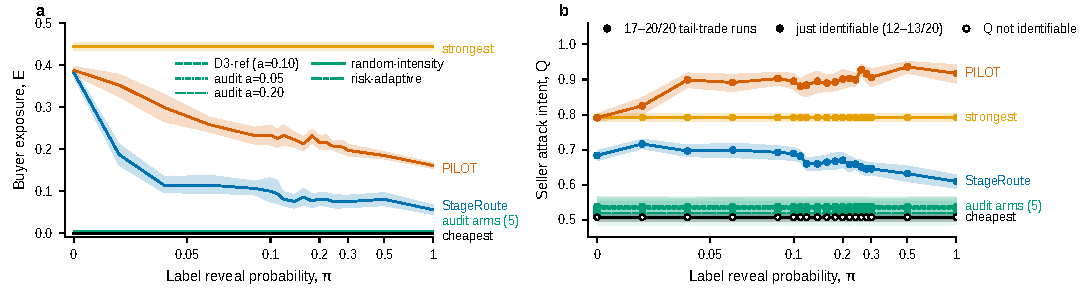
\includegraphics[width=\textwidth]{figures/fig3_40seller_E_Q_vs_pi.pdf}
  \caption{Buyer exposure $\Emet$ (a) and seller intent $\Qmet$ (b) vs.\ reveal probability $\pi$ at 40 sellers. Lines are means over $n=20$ seeds; bands are 95\% paired-bootstrap CIs (10,000 resamples). The five audit arms share one colour and differ by line style. $\pi$ axis: symlog, linear below 0.08. $\Qmet$ markers: solid 17--20/20 tail-trade runs; half-filled 12--13/20 (audits, just identifiable); hollow 0/20 (cheapest). Audit and fixed-router curves are flat in $\pi$ by construction and are not reported as a finding.}
  \Description{Two line charts against reveal probability pi at 40 sellers. Left: E for PILOT and StageRoute rises as pi falls and the two are close at pi = 0; cheapest stays at 0; strongest is flat near 0.45; audit arms are flat near 0. Right: Q for PILOT stays high and dips only at the lowest pi; StageRoute Q, drawn solid, rises as pi falls; cheapest Q is hollow throughout; audit arms are flat and drawn half-filled (just identifiable, 12-13 of 20 runs).}
  \label{fig:t2}
\end{figure*}

\paragraph{Reading.} At 40 sellers, $\Emet$ of both bandit routers is significantly worse at every $\pi<1$ than at $\pi=1$ (paired, Holm over $\pi$). StageRoute's $\Qmet$ is identifiable (tail-trade runs 85--100\%) and is significantly higher at every lower $\pi$ than at $\pi=1$. PILOT always has 20/20 tail-trade runs; its $\Emet$ is significantly worse at every lower $\pi$, while for $\pi\ge 0.04$ its $\Qmet$ is 0.88--0.94 with no significant rise vs.\ $\pi=1$, and is significantly lower only at $\pi=0$ (0.791) and $\pi=0.02$ (0.825); we do not interpret this as deterrence. At $\pi=0$, PILOT and StageRoute $\Emet$ are already close and not significantly different: $+0.006$ [$-0.007$, $+0.019$], $p_{\mathrm{Holm}}=1.0$. Cheapest remains at $\Emet=0$ with $\Qmet$ not identifiable. The v1.0 48-round audit arms are as in Appendix~\ref{app:t1-v10} (low $\Emet$ by rare trade with strategic sellers, not deterrence); their flatness in $\pi$ is by construction. The $J$ crossover is an appendix result; under the pre-registered rule the interval $(0.10,0.12)$ is not kept.

\subsection{T4 --- Seller risk ranking}
\label{sec:t4}
Under the official D3 setting at $\pi=1$ with a resampled roster, the test set has only two positives among 89 scored sellers (those who traded in the target window, not all 40 on each roster), and only two of six test runs have both classes. We therefore do not report detection performance and do not interpret the latency ablation; a pooled-over-sellers calculation, which does not follow the protocol, is noted in Appendix~\ref{app:secondary}.

A PILOT, $\pi=1$ supplement on the current simulator (before the 5b change), with the same split and a resampled roster, is scorable (6/6 test runs) but is not a new official main result; we do not read it as detection already succeeding or as buyers generally detecting fraud. Positives in this batch (49/215; $\Emet=0.158$) come from PILOT still trading with strategic sellers, not from solving scarce positives under D3, and not a general claim that trading with attackers makes detection scorable. Table~\ref{tab:t4pilot}: \code{any} logistic AUROC $0.970$ [$0.941$, $0.991$], $0.895$ without latency (above the rule $0.703$ in all six test runs; this setting only, not equally strong without latency); latency contributes on \code{any} but not for every attack type, and types must not be collapsed into a single $0.97$.

\subsection{A2 --- Compliance control}
\label{sec:a2}
With the filter off at $\pi=1$ over seeds 0--19 (Table~\ref{tab:a2}), every method's violation rate rises significantly from 0 (PILOT 0.156 [0.152, 0.159], StageRoute 0.178 [0.169, 0.188], cheapest 0.065 [0.062, 0.068], strongest 0.191 [0.185, 0.197], D3-ref and the other audit arms $\approx$0.166--0.167). Fill rates have no significant change after Holm. The zeros in the v1.0 baseline table therefore come from the filter, not from an absence of violating buyer--seller pairs. The D3 filter-off arm is \code{fixed_audit_a0.10} with \code{--no-compliance-filter}. $\Emet$ of PILOT, StageRoute, and cheapest does not change significantly; strongest rises significantly (0.446$\rightarrow$0.519). The audit $\Emet$ dip is significant, but with the filter off their tail-trade runs fall to 1/20, so $\Qmet$ is not identifiable---we do not report those $\Qmet$ values, and we do not read the dip as a reduction in attacks from turning the filter off. StageRoute's filter-off tail-trade runs are 11/20, just over the identifiability line, and $\Qmet$ is almost unchanged; we draw no strong reading. This control is only at $\pi=1$.

\begin{table}[!htbp]
\caption{A2 filter control, 40 sellers, $\pi=1$, seeds 0--19, paired (mean [95\% CI]). Viol.\ ON $=0$ for every method. Fill-rate off$-$on differences are all Holm-n.s.\ (not shown). D3 OFF is \texttt{fixed\_audit\_a0.10} with \texttt{--no-compliance-filter}. Audit filter-off $\Qmet$ omitted (1/20 tail trades, not identifiable).}
\label{tab:a2}
\scriptsize
\setlength{\tabcolsep}{2.2pt}
\renewcommand{\arraystretch}{0.9}
\begin{tabular}{@{}lcccc@{}}
\toprule
Policy & Viol.\ OFF & $\Emet$ ON & $\Emet$ OFF & Tail ON / OFF \\
\midrule
PILOT & \cil{0.156}{0.152}{0.159} & \cil{0.161}{0.154}{0.168} & \cil{0.159}{0.154}{0.164} & 20/20 / 20/20 \\
StageRoute & \cil{0.178}{0.169}{0.188} & \cil{0.056}{0.045}{0.068} & \cil{0.050}{0.036}{0.066} & 17/20 / 11/20 \\
Cheapest & \cil{0.065}{0.062}{0.068} & \cil{0.000}{0.000}{0.000} & \cil{0.000}{0.000}{0.000} & 0/20 / 0/20 \\
Strongest & \cil{0.191}{0.185}{0.197} & \cil{0.446}{0.436}{0.455} & \cil{0.519}{0.512}{0.526} & 20/20 / 20/20 \\
Random-intensity & \cil{0.166}{0.159}{0.173} & \cil{0.005}{0.004}{0.005} & \cil{0.001}{0.001}{0.002} & 13/20 / 1/20 \\
Fixed-rate $a=0.05$ & \cil{0.167}{0.160}{0.174} & \cil{0.005}{0.004}{0.006} & \cil{0.001}{0.001}{0.002} & 13/20 / 1/20 \\
D3-ref ($a=0.1$) & \cil{0.166}{0.159}{0.173} & \cil{0.005}{0.004}{0.006} & \cil{0.001}{0.001}{0.002} & 13/20 / 1/20 \\
Fixed-rate $a=0.2$ & \cil{0.167}{0.161}{0.174} & \cil{0.004}{0.003}{0.005} & \cil{0.001}{0.001}{0.002} & 13/20 / 1/20 \\
Risk-adaptive & \cil{0.166}{0.159}{0.172} & \cil{0.005}{0.004}{0.006} & \cil{0.001}{0.001}{0.002} & 12/20 / 1/20 \\
\bottomrule
\end{tabular}
\end{table}
%% =====================================================================
\section{Limitations}
\label{sec:limitations}

\begin{enumerate}
\item \textbf{Single-platform auditor; no multi-buyer congestion.} Multi-buyer competition for capacity and multi-auditor games are deferred. Congestion externalities are outside the leaderboard contract.
\item \textbf{Not a CLOB.} Posted prices + routing/portfolio procurement only; no price--time priority book, maker--taker fees, HFT makers, or circuit breakers.
\item \textbf{Synthetic jurisdictions and mechanism + cached model answers.} Corridor tags (CN/SG/BR) and compliance profiles are simplified simulation devices---not legal advice and not real KYC/data-transfer regimes. Correctness comes from cached generations of a small set of models; prices, budgets, audits, and learning rules are simulated; calibration of prices to public list prices is \TBD{Coding: price sources and mapping}.
\item \textbf{$\Qmet$ depends on the seller learning rule and on trading.} For v1.0, it is primary only if it passes the learning-rule gate (\S\ref{sec:metrics}); Decision A uses its separate direction rule. It is not identifiable for sellers that a router avoids completely.
\item \textbf{T4 realism.} Before the 5b change, the simulator does not separate hidden reasoning from visible answers, so several realistic buyer signals (answer length, quality) are excluded for leakage; latency may be more revealing than in real markets, hence the without-latency ablation.
\item \textbf{Simulation-only audit effect.} Decision A shows an audit effect only in this simulator under default parameters ($P=0.25$, $\pi=1$), 1000 rounds, and the three seller rules (egreedy, fictitious play, EXP3). EXP3 keeps $\Qmet\approx0.5$; PILOT $\Emet$ has no significant change and $\Qmet$ decreases are small. This does not establish effects in real API markets or deployments. T3's equal-budget adaptive comparison and long delist remain optional knobs.
\item \textbf{No resale / rewrite / distill event graph.} No \code{event_type}$\in$\{\code{resale},\code{rewrite},\code{distill}\} layer, parent/source order links, or content/output hashes; strong provenance is deferred to a later event layer.
\end{enumerate}

%% =====================================================================
\section{Conclusion}
\label{sec:conclusion}

We release a \textbf{compliance-constrained reasoning-token market simulator}---a \textbf{generator + protocol + downloadable board}, not a new routing, audit, or detection method---for procurement under strategic fraud and sparse audit feedback. The platform is deliberately \emph{not} a CLOB: it exposes admission, routing, escrow, oversight, and feedback trails as a joinable five-file export with a leakage-checked feature view. Evaluation is two-dimensional (buyer exposure $\Emet$, seller intent $\Qmet$) and reported as a Pareto plot without a declared winner. At 40 sellers, both bandit routers' $\Emet$ rises significantly as labels vanish; StageRoute's $\Qmet$ is identifiable and rises as $\pi$ falls, while PILOT's $\Qmet$ does not rise relative to $\pi=1$ (and is lower only at $\pi=0$ and $0.02$). The v1.0 48-round audit arms sit at low $\Emet$ mainly by rarely trading with strategic sellers, which is not read as deterrence. In this simulator, under default parameters at 1000 rounds, audits lower $\Emet$ and $\Qmet$ separately for PILOT and strongest by the pre-run egreedy/fictitious-play/EXP3 rule (result 1) (with the EXP3 caveat in \S\ref{sec:t1}). T4 is defined, but under the official D3 setting the test set has only two positives and most test runs cannot yield a per-protocol AUROC, so we do not report detection performance. A PILOT, $\pi=1$ supplement is scorable and is reported in \S\ref{sec:t4}; it is not a new official main result. Designing methods that move the Pareto front is left to future work. We invite leaderboard entries on T1, T2, and T4, with T3 and delist kept as cost/ops appendices.

%% =====================================================================
\section*{Ethics and Synthetic-Data Statement}
\label{sec:ethics}

Budgets, stakes, corridor fees, and compliance rule identifiers are \textbf{synthetic}; list prices are intended to be calibrated to public API price lists (\TBD{Coding: price sources, access date, calibration}); no real transaction data is used. Jurisdiction labels (CN/SG/BR) and rule tags are simplified simulation devices and \textbf{do not constitute legal advice}. Benchmark runs do not call external commercial APIs or require API keys; cached model outputs are research fixtures. The benchmark is intended for studying procurement, audit, and feedback protocols---not for training systems to evade real-world marketplace detection. Users building fraud classifiers must respect the Feature/Label separation in \S\ref{sec:featlabel} to avoid leakage and overstated detection performance.

%% =====================================================================
\FloatBarrier
\nocite{bester2001strategic,cumming2019capital}
\bibliographystyle{ACM-Reference-Format}
\bibliography{refs}

%% =====================================================================
\appendix

\section{Schema field cheat-sheet}
\label{app:schema}

See \code{docs/DATA_SCHEMA.md} for full dictionaries and three-row samples. Minimal board row (\code{episodes.jsonl}): \code{run_id, seed, a, pi, L, reputation_rounds, fraud_share} ($\Emet$), $\Qmet$, per-mode learned $q$ over listed rounds, suspended rounds and suspended-period $q$, \code{J, n_audits, config_hash} (final field names: \TBD{Coding: v1.0 episodes field names}). \code{active_attack_rate} is removed (same formula as \code{fraud_share}).

\section{Reproducibility and Artifact Paths}
\label{app:repro}

All repository and file paths referenced by the main text are collected here. The v1.0 release pack \code{release/v1.0/} is self-contained: \code{LICENSE} (MIT) and data license notes (CC BY 4.0), \code{LICENSES/DATA_LICENSES.md}, \code{requirements.txt}, \code{REPRODUCE.md}, a \code{MANIFEST} with sha256 sums, a data card, the LLM output cache, and all v1.0 results. The frozen \code{release/v0.1/} is kept unchanged for history; v1.0 results are not written into it.

\paragraph{One-click scripts.}
\begin{lstlisting}
# Production board (-> exports/production/)
python scripts/export_benchmark_layers.py --full --use-cache --out exports/production
# Protocol tasks (production scale)
python scripts/run_benchmark_tasks.py --full --use-cache
# Dense pi grid, per-seed tables
scripts/reproduce_pi_dense.sh --full
\end{lstlisting}
v1.0 commands for T4, the leakage check, and the per-seed option: \TBD{Coding: final v1.0 command lines}.

\begin{table*}[h]
\caption{Reproducibility summary (v1.0 and T1 v1.2 Decision A).}
\label{tab:repro}
\small
\begin{tabularx}{\textwidth}{@{}l X@{}}
\toprule
Item & Value / path \\
\midrule
Downloadable pack & \code{release/v1.0/} (\code{MANIFEST}, \code{MANIFEST.json}, \code{REPRODUCE.md}, \code{LICENSE_NOTES.md}, \code{LICENSES/}) \\
Protocol & \code{docs/PROTOCOL_v1.0.md} (frozen before the 40-seller main table; post-batch clarifications in App.~\ref{app:amend}) \\
Production board & \code{release/v1.0/exports/production/}\{\code{sellers},\code{buyers},\code{orders},\code{audits},\code{episodes}\}\code{.jsonl} + held-out labels \\
T1--T4 results & \code{results/v1.0/} $\rightarrow$ \code{release/v1.0/results/} \\
Decision A readout & \code{results/v1.1/v1.2_decision_a_eval/}, commit \code{f759cd6}; \code{decision_a_eval.md} sha256 \code{5d3f52292883a73dec8a892e7e64c250eeb7eb62c09b1bb36508e7e3c034dad9} (verified against its \code{.sha256}) \\
Decision A protocol & \code{docs/v1.1/PROTOCOL_v1.2.md}, sha256 \code{daddac6c0dddb22b08701caff5715e77215ae13a588512af176ff4933430b102} \\
Decision A table generation & \code{python3 scripts/pass12_decision_a_tables.py} $\rightarrow$ \code{docs/latex-sigkdd-v1.0/tables/decision_a_*.tex} \\
Dense $\pi$ grid & \code{configs/pi_dense.yaml} (v1.0 grid: \TBD{Coding: v1.0 config path}) $\rightarrow$ \code{release/v1.0/results/pi_dense/} \\
First v1.0 batch (v0.1 scale) & \code{results/v1.0/T2_v01scale_20seed.\{md,json\}}, \code{A2_compliance_control.\{md,json\}}, \code{Q_gate_v01scale.json}, \code{regression_gate_seed0-2.json}, \code{raw/*.jsonl}; scripts \code{scripts/v1/} \\
40-seller main table (egreedy) & \code{results/v1.0/main/} (\code{inference.md}, \code{inference.json}, \code{summary.md}) \\
Q-gate peer (fictitious play) & \code{results/v1.0/main_fp/} \\
Q averaging / gate robustness & \code{results/v1.0/main/Q_tail_only_robustness.md} \\
A2 filter-off & \code{results/v1.0/a2_filter_off/} (\code{A2_paired.md}, \code{A2_paired.json}) \\
EXP3 appendix & \code{results/v1.0/main_exp3/} \\
T4 official (D3, $\pi=1$) & \code{results/v1.0/t4_eval/} (export, unchanged) and \code{results/v1.0/t4_eval_per_run/} (per-run official recompute) \\
T4 supplement (PILOT, $\pi=1$) & \code{results/v1.0/t4_pilot_eval/} \\
Frozen scale config & \code{configs/v1.0/frozen/scale.yaml}, sha256 \code{780e9b961d89bad6fd520c9cbfd5710055ff2d5d3e0ff3bcfbd745709eb0da6c} \\
LLM output cache & \code{release/v1.0/cache/llm_outputs.jsonl} (+ \code{CACHE_MANIFEST.json}) \\
Feature/Label rules & \code{docs/DATA_SCHEMA.md}, \S\ref{sec:featlabel}, leakage check \TBD{Coding: script path} \\
Seeds & $\ge$20 (main table); T4 train 0--13, test 14--19 \\
Production \code{config_hash} & \TBD{Coding: v1.0 config hash} \\
Default knobs & \code{adaptive_audit=false}, \code{reputation_rounds=0}, \code{escrow=false} \\
Test suite & \TBD{Coding: v1.0 pytest count and log path} \\
\bottomrule
\end{tabularx}
\end{table*}

\begin{table}[h]
\caption{Platform layer code map.}
\label{tab:codemap}
\small
\begin{tabularx}{\columnwidth}{@{}l X@{}}
\toprule
Layer & Code map \\
\midrule
1. Admission / compliance & \code{gateway.py}, \code{compliance.py} \\
2. Routing / portfolio & \code{matching.py}, \code{portfolio.py}, \code{buyers.py}, \code{baselines.py} \\
3. Escrow settlement & \code{sim.py}, \code{audit_v6.py} \\
4. Oversight & \code{strategic.py}, \code{audit_v6.py} \\
5. Feedback \& trails & \code{feedback.py}, \code{logging_schema.py} \\
\bottomrule
\end{tabularx}
\end{table}

\section{Decision A paired contrasts (v1.2)}
\label{app:decision-a}

Tables~\ref{tab:decision-a-pilot} and~\ref{tab:decision-a-strongest} contain every default-parameter paired contrast behind Table~\ref{tab:t1}; no learner is dropped. Means and significance markers are generated from \code{cells.csv} and \code{contrasts.csv}, with the result-1 votes checked against \code{direction_consistency.csv}. Lower-penalty cells remain in the official machine-readable readout: $P/4$ has frozen $a^*\approx0.18$--$0.20$; $P/16$ has $a^*\approx0.71$--$0.80$ and is descriptive only, never evidence of audit efficacy. All default cells have 20/20 tail-trade runs. These results use identity+length and \code{trust_feedback=false}; they are not direct numerical comparisons with v1.0 audit arms.

% Generated by scripts/pass12_decision_a_tables.py; do not edit.

\begin{table*}[p]
\caption{Decision A, PILOT: full paired audit-minus-$a=0$ deltas at $P=0.25$, $\pi=1$, 1000 rounds, seeds 0--19. Intervals: 95\% same-seed paired-bootstrap percentile CIs, $B=10{,}000$; $p_{\mathrm{raw}}$ is two-sided, $p_{\mathrm{H}}$ uses the merged 84-test Holm family. $^{*}$: significant decrease ($p_{\mathrm{H}}<0.05$). Values below the bootstrap floor are written $<10^{-4}$. $^{\dagger}$: $a=0.05$ is the upper edge of $a^*=[0.044,0.050]$. $a=0.01$--$0.03$ are below $a^*$ and not counted toward result 1. Rounding to three decimals can mask tiny changes or CI endpoints.}
\label{tab:decision-a-pilot}
\centering\footnotesize
\setlength{\tabcolsep}{4pt}
\renewcommand{\arraystretch}{0.90}
\begin{tabular}{@{}lcccccc@{}}
\toprule
Audit $a$ & $\Delta\Emet$ [95\% CI] & $p_{\mathrm{raw}}$ & $p_{\mathrm{H}}$ & $\Delta\Qmet$ [95\% CI] & $p_{\mathrm{raw}}$ & $p_{\mathrm{H}}$ \\
\midrule
\multicolumn{7}{l}{egreedy} \\
0.01 & $-0.010\;[-0.016, -0.005]$$^{*}$ & $<10^{-4}$ & $<10^{-4}$ & $-0.113\;[-0.151, -0.075]$$^{*}$ & $<10^{-4}$ & $<10^{-4}$ \\
0.02 & $-0.030\;[-0.040, -0.021]$$^{*}$ & $<10^{-4}$ & $<10^{-4}$ & $-0.254\;[-0.311, -0.194]$$^{*}$ & $<10^{-4}$ & $<10^{-4}$ \\
0.03 & $-0.039\;[-0.048, -0.030]$$^{*}$ & $<10^{-4}$ & $<10^{-4}$ & $-0.331\;[-0.377, -0.287]$$^{*}$ & $<10^{-4}$ & $<10^{-4}$ \\
0.05$^{\dagger}$ & $-0.075\;[-0.081, -0.068]$$^{*}$ & $<10^{-4}$ & $<10^{-4}$ & $-0.563\;[-0.617, -0.506]$$^{*}$ & $<10^{-4}$ & $<10^{-4}$ \\
0.10 & $-0.089\;[-0.093, -0.085]$$^{*}$ & $<10^{-4}$ & $<10^{-4}$ & $-0.758\;[-0.804, -0.709]$$^{*}$ & $<10^{-4}$ & $<10^{-4}$ \\
0.20 & $-0.095\;[-0.098, -0.092]$$^{*}$ & $<10^{-4}$ & $<10^{-4}$ & $-0.862\;[-0.885, -0.834]$$^{*}$ & $<10^{-4}$ & $<10^{-4}$ \\
risk-adaptive & $-0.089\;[-0.092, -0.085]$$^{*}$ & $<10^{-4}$ & $<10^{-4}$ & $-0.725\;[-0.767, -0.682]$$^{*}$ & $<10^{-4}$ & $<10^{-4}$ \\
\midrule
\multicolumn{7}{l}{fictitious play} \\
0.01 & $-0.007\;[-0.012, -0.003]$$^{*}$ & $0.0016$ & $0.0224$ & $-0.062\;[-0.093, -0.035]$$^{*}$ & $<10^{-4}$ & $<10^{-4}$ \\
0.02 & $-0.028\;[-0.038, -0.018]$$^{*}$ & $<10^{-4}$ & $<10^{-4}$ & $-0.201\;[-0.270, -0.141]$$^{*}$ & $<10^{-4}$ & $<10^{-4}$ \\
0.03 & $-0.046\;[-0.054, -0.037]$$^{*}$ & $<10^{-4}$ & $<10^{-4}$ & $-0.328\;[-0.387, -0.269]$$^{*}$ & $<10^{-4}$ & $<10^{-4}$ \\
0.05$^{\dagger}$ & $-0.064\;[-0.073, -0.055]$$^{*}$ & $<10^{-4}$ & $<10^{-4}$ & $-0.473\;[-0.518, -0.429]$$^{*}$ & $<10^{-4}$ & $<10^{-4}$ \\
0.10 & $-0.099\;[-0.103, -0.094]$$^{*}$ & $<10^{-4}$ & $<10^{-4}$ & $-0.707\;[-0.741, -0.672]$$^{*}$ & $<10^{-4}$ & $<10^{-4}$ \\
0.20 & $-0.108\;[-0.112, -0.104]$$^{*}$ & $<10^{-4}$ & $<10^{-4}$ & $-0.804\;[-0.821, -0.786]$$^{*}$ & $<10^{-4}$ & $<10^{-4}$ \\
risk-adaptive & $-0.099\;[-0.103, -0.094]$$^{*}$ & $<10^{-4}$ & $<10^{-4}$ & $-0.691\;[-0.726, -0.655]$$^{*}$ & $<10^{-4}$ & $<10^{-4}$ \\
\midrule
\multicolumn{7}{l}{EXP3} \\
0.01 & $+0.000\;[-0.000, +0.001]$ & $0.4018$ & $1.0000$ & $-0.000\;[-0.001, +0.001]$ & $0.9462$ & $1.0000$ \\
0.02 & $+0.000\;[-0.001, +0.001]$ & $0.7382$ & $1.0000$ & $-0.000\;[-0.001, +0.000]$ & $0.2772$ & $1.0000$ \\
0.03 & $-0.000\;[-0.001, +0.001]$ & $0.8242$ & $1.0000$ & $-0.001\;[-0.002, -0.000]$ & $0.0336$ & $0.4032$ \\
0.05$^{\dagger}$ & $-0.000\;[-0.001, +0.001]$ & $0.6296$ & $1.0000$ & $-0.003\;[-0.004, -0.002]$$^{*}$ & $<10^{-4}$ & $<10^{-4}$ \\
0.10 & $+0.001\;[-0.001, +0.003]$ & $0.3114$ & $1.0000$ & $-0.004\;[-0.005, -0.002]$$^{*}$ & $<10^{-4}$ & $<10^{-4}$ \\
0.20 & $+0.001\;[-0.001, +0.003]$ & $0.2810$ & $1.0000$ & $-0.009\;[-0.012, -0.006]$$^{*}$ & $<10^{-4}$ & $<10^{-4}$ \\
risk-adaptive & $-0.001\;[-0.002, +0.001]$ & $0.3962$ & $1.0000$ & $-0.009\;[-0.011, -0.007]$$^{*}$ & $<10^{-4}$ & $<10^{-4}$ \\
\bottomrule
\end{tabular}
\end{table*}
\begin{table*}[p]
\caption{Decision A, strongest: full paired audit-minus-$a=0$ deltas at $P=0.25$, $\pi=1$, 1000 rounds, seeds 0--19. Intervals: 95\% same-seed paired-bootstrap percentile CIs, $B=10{,}000$; $p_{\mathrm{raw}}$ is two-sided, $p_{\mathrm{H}}$ uses the merged 84-test Holm family. $^{*}$: significant decrease ($p_{\mathrm{H}}<0.05$). Values below the bootstrap floor are written $<10^{-4}$. $^{\dagger}$: $a=0.05$ is the upper edge of $a^*=[0.044,0.050]$. $a=0.01$--$0.03$ are below $a^*$ and not counted toward result 1. Rounding to three decimals can mask tiny changes or CI endpoints.}
\label{tab:decision-a-strongest}
\centering\footnotesize
\setlength{\tabcolsep}{4pt}
\renewcommand{\arraystretch}{0.90}
\begin{tabular}{@{}lcccccc@{}}
\toprule
Audit $a$ & $\Delta\Emet$ [95\% CI] & $p_{\mathrm{raw}}$ & $p_{\mathrm{H}}$ & $\Delta\Qmet$ [95\% CI] & $p_{\mathrm{raw}}$ & $p_{\mathrm{H}}$ \\
\midrule
\multicolumn{7}{l}{egreedy} \\
0.01 & $-0.018\;[-0.031, -0.008]$$^{*}$ & $<10^{-4}$ & $<10^{-4}$ & $-0.006\;[-0.017, +0.000]$ & $0.2476$ & $1.0000$ \\
0.02 & $-0.122\;[-0.163, -0.083]$$^{*}$ & $<10^{-4}$ & $<10^{-4}$ & $-0.101\;[-0.139, -0.066]$$^{*}$ & $<10^{-4}$ & $<10^{-4}$ \\
0.03 & $-0.189\;[-0.229, -0.148]$$^{*}$ & $<10^{-4}$ & $<10^{-4}$ & $-0.173\;[-0.222, -0.126]$$^{*}$ & $<10^{-4}$ & $<10^{-4}$ \\
0.05$^{\dagger}$ & $-0.317\;[-0.344, -0.289]$$^{*}$ & $<10^{-4}$ & $<10^{-4}$ & $-0.409\;[-0.454, -0.367]$$^{*}$ & $<10^{-4}$ & $<10^{-4}$ \\
0.10 & $-0.424\;[-0.428, -0.419]$$^{*}$ & $<10^{-4}$ & $<10^{-4}$ & $-0.593\;[-0.599, -0.584]$$^{*}$ & $<10^{-4}$ & $<10^{-4}$ \\
0.20 & $-0.435\;[-0.436, -0.433]$$^{*}$ & $<10^{-4}$ & $<10^{-4}$ & $-0.600\;[-0.603, -0.598]$$^{*}$ & $<10^{-4}$ & $<10^{-4}$ \\
risk-adaptive & $-0.419\;[-0.424, -0.414]$$^{*}$ & $<10^{-4}$ & $<10^{-4}$ & $-0.581\;[-0.595, -0.562]$$^{*}$ & $<10^{-4}$ & $<10^{-4}$ \\
\midrule
\multicolumn{7}{l}{fictitious play} \\
0.01 & $-0.044\;[-0.084, -0.015]$$^{*}$ & $<10^{-4}$ & $<10^{-4}$ & $-0.052\;[-0.089, -0.025]$$^{*}$ & $<10^{-4}$ & $<10^{-4}$ \\
0.02 & $-0.145\;[-0.196, -0.097]$$^{*}$ & $<10^{-4}$ & $<10^{-4}$ & $-0.177\;[-0.220, -0.136]$$^{*}$ & $<10^{-4}$ & $<10^{-4}$ \\
0.03 & $-0.199\;[-0.253, -0.148]$$^{*}$ & $<10^{-4}$ & $<10^{-4}$ & $-0.252\;[-0.302, -0.201]$$^{*}$ & $<10^{-4}$ & $<10^{-4}$ \\
0.05$^{\dagger}$ & $-0.323\;[-0.356, -0.287]$$^{*}$ & $<10^{-4}$ & $<10^{-4}$ & $-0.416\;[-0.456, -0.376]$$^{*}$ & $<10^{-4}$ & $<10^{-4}$ \\
0.10 & $-0.422\;[-0.431, -0.413]$$^{*}$ & $<10^{-4}$ & $<10^{-4}$ & $-0.569\;[-0.583, -0.557]$$^{*}$ & $<10^{-4}$ & $<10^{-4}$ \\
0.20 & $-0.462\;[-0.464, -0.460]$$^{*}$ & $<10^{-4}$ & $<10^{-4}$ & $-0.631\;[-0.634, -0.628]$$^{*}$ & $<10^{-4}$ & $<10^{-4}$ \\
risk-adaptive & $-0.422\;[-0.431, -0.413]$$^{*}$ & $<10^{-4}$ & $<10^{-4}$ & $-0.564\;[-0.579, -0.550]$$^{*}$ & $<10^{-4}$ & $<10^{-4}$ \\
\midrule
\multicolumn{7}{l}{EXP3} \\
0.01 & $-0.000\;[-0.001, +0.000]$ & $0.1648$ & $1.0000$ & $-0.001\;[-0.001, -0.001]$$^{*}$ & $<10^{-4}$ & $<10^{-4}$ \\
0.02 & $-0.001\;[-0.002, -0.000]$ & $0.0072$ & $0.0936$ & $-0.002\;[-0.002, -0.001]$$^{*}$ & $<10^{-4}$ & $<10^{-4}$ \\
0.03 & $-0.001\;[-0.002, -0.000]$$^{*}$ & $0.0004$ & $0.0060$ & $-0.003\;[-0.003, -0.002]$$^{*}$ & $<10^{-4}$ & $<10^{-4}$ \\
0.05$^{\dagger}$ & $-0.003\;[-0.004, -0.003]$$^{*}$ & $<10^{-4}$ & $<10^{-4}$ & $-0.005\;[-0.005, -0.004]$$^{*}$ & $<10^{-4}$ & $<10^{-4}$ \\
0.10 & $-0.006\;[-0.007, -0.005]$$^{*}$ & $<10^{-4}$ & $<10^{-4}$ & $-0.009\;[-0.010, -0.009]$$^{*}$ & $<10^{-4}$ & $<10^{-4}$ \\
0.20 & $-0.012\;[-0.013, -0.010]$$^{*}$ & $<10^{-4}$ & $<10^{-4}$ & $-0.019\;[-0.020, -0.018]$$^{*}$ & $<10^{-4}$ & $<10^{-4}$ \\
risk-adaptive & $-0.012\;[-0.014, -0.011]$$^{*}$ & $<10^{-4}$ & $<10^{-4}$ & $-0.019\;[-0.020, -0.018]$$^{*}$ & $<10^{-4}$ & $<10^{-4}$ \\
\bottomrule
\end{tabular}
\end{table*}

\FloatBarrier

\section{v1.0 48-round baseline Pareto view}
\label{app:t1-v10}

The following preserves the v1.0 setting and interpretation: 48 rounds, egreedy, identity-only checks on non-cascade paths, identity+length on cascade audit arms. It is distinct from the v1.2 router $\times$ audit experiment.

\begin{table*}[t]
\caption{v1.0 48-round baseline Pareto view (identity-only non-cascade checks; cascade audit arms use identity+length), at $\pi=1$, $L=0$, 40 sellers, 20 seeds (mean [95\% CI]). Primary: $\Emet$ (per purchase) and $\Qmet$. Side: billed-token-weighted $\Emet_{\mathrm{tok}}$. $\Qmet$ stays primary because the fictitious-play gate just passes (Kendall $\tau_a=0.643$). Rows are not ranked. $^{\circ}$: $\Qmet$ not identifiable (tail-trade runs $\le$50\%). Per-mode $q$ and $J$: Appendix~\ref{app:secondary}.}
\label{tab:t1-v10}
\footnotesize
\setlength{\tabcolsep}{4pt}
\renewcommand{\arraystretch}{0.95}
\begin{tabular}{@{}lcccc@{}}
\toprule
Policy & $\Emet$ & $\Emet_{\mathrm{tok}}$ (side) & $\Qmet$ & Tail-trade runs \\
\midrule
PILOT (faithful) + compliance & \cil{0.161}{0.154}{0.168} & \cil{0.178}{0.169}{0.186} & \cil{0.917}{0.890}{0.942} & 20/20 \\
StageRoute (faithful, MIP) + compliance & \cil{0.056}{0.044}{0.068} & \cil{0.065}{0.052}{0.078} & \cil{0.609}{0.590}{0.628} & 17/20 \\
Fixed router (cheapest) & \cil{0.000}{0.000}{0.000} & \cil{0.000}{0.000}{0.000} & \cil{0.508}{0.495}{0.520}$^{\circ}$ & 0/20 \\
Fixed router (strongest) & \cil{0.446}{0.436}{0.455} & \cil{0.495}{0.485}{0.505} & \cil{0.792}{0.779}{0.804} & 20/20 \\
Fixed-rate audit $a=0.05$ & \cil{0.005}{0.004}{0.006} & \cil{0.006}{0.005}{0.008} & \cil{0.531}{0.501}{0.559} & 13/20 \\
D3-ref / fixed-rate audit $a=0.1$ & \cil{0.005}{0.004}{0.006} & \cil{0.006}{0.005}{0.007} & \cil{0.538}{0.508}{0.566} & 13/20 \\
Fixed-rate audit $a=0.2$ & \cil{0.004}{0.003}{0.005} & \cil{0.006}{0.004}{0.007} & \cil{0.519}{0.485}{0.552} & 13/20 \\
Random-intensity audit & \cil{0.005}{0.004}{0.005} & \cil{0.006}{0.005}{0.007} & \cil{0.533}{0.500}{0.563} & 13/20 \\
Risk-adaptive audit & \cil{0.005}{0.004}{0.006} & \cil{0.006}{0.005}{0.007} & \cil{0.536}{0.504}{0.565} & 12/20 \\
\bottomrule
\end{tabular}
\end{table*}

\begin{figure}[t]
  \centering
  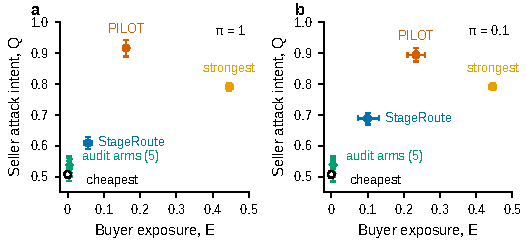
\includegraphics[width=\linewidth]{figures/fig2_40seller_pareto_EQ.pdf}
  \caption{v1.0 48-round baseline Pareto view: $(\Emet,\Qmet)$ at $\pi=1$ (a) and $\pi=0.1$ (b), 40 sellers. Points are means over $n=20$ seeds; bars are 95\% paired-bootstrap CIs (10,000 resamples). The five audit arms share one colour and overlap at low $\Emet$ (values in Table~\ref{tab:t1-v10}). Solid: 17--20/20 tail-trade runs; half-filled: audits (12--13/20); cheapest is hollow (0/20) and is not on the two-dimensional front---read it along $\Emet$ only. Front membership is not concluded; no winner is declared.}
  \Description{Two scatter panels of buyer exposure E against seller intent Q at pi = 1 and pi = 0.1 for nine methods, with interval bars. Cheapest is a hollow marker at E = 0. The five audit arms cluster and overlap at low E and are drawn half-filled (just identifiable, 12-13 of 20 runs). StageRoute and PILOT are solid (identifiable) in both panels. No point is highlighted as a front.}
  \label{fig:pareto}
\end{figure}

\paragraph{Reading (v1.0, 48 rounds).} The fictitious-play gate is a pre-run mechanical rule and just passes: 8 identifiable methods under both egreedy and fictitious play, at every $\pi$, Kendall $\tau_a=0.643$ (23 concordant pairs, 5 discordant), just over 0.6. We do not call this ordering stable. Identifiable points are plotted with interval bars (Figure~\ref{fig:pareto}); we do not declare a Pareto-front winner, and front membership from point estimates is not reported as a finding. Cheapest has the best $\Emet=0$ but $\Qmet$ is not identifiable (0/20 tail-trade runs), so it does not enter the two-dimensional front and is read along $\Emet$ only. At $\pi=1$, differences in $\Emet$ and $\Qmet$ between $a=0.20$ and the D3 reference, random-intensity, and risk-adaptive arms either have intervals containing 0 or fail Holm, so those audit arms are not separable. Audit $\Qmet$ just clears the identifiability line (12--13/20 tail-trade runs; risk-adaptive 12/20, the others 13/20) and is not read as deterrence. Their $\Emet$ is very low ($\approx$0.004--0.005) mainly because they rarely trade with strategic sellers, not because of deterrence. This holds only under the v1.0 48-round setting's audit and slashing parameters; it does not describe the v1.2 1000-round Decision A grid.

\FloatBarrier

\section{Secondary results}
\label{app:secondary}

\paragraph{$J$ and $\Emet_{\mathrm{tok}}$ (v1.0 48-round setting, $\pi=1$).}
Table~\ref{tab:j} reports the joint objective $J$ (mean [95\% CI], 20 seeds). Cost and quality intervals are not in the official inference file: \TBD{T1-secondary: cost and accuracy per policy, mean [95\% CI]}. $\Emet_{\mathrm{tok}}$ is the billed-token-weighted side column of the v1.0 Table~\ref{tab:t1-v10}; Figure~\ref{fig:etok} shows the same 19-point $\pi$ sweep. The primary $\Emet$ stays per purchase.

\begin{table}[h]
\caption{Appendix $J$ at $\pi=1$, $L=0$, 40 sellers, 20 seeds (mean [95\% CI]). Not used to rank methods in the body.}
\label{tab:j}
\footnotesize
\begin{tabular}{@{}lc@{}}
\toprule
Policy & $J$ \\
\midrule
PILOT (faithful) + compliance & 0.706 [0.699, 0.714] \\
StageRoute (faithful, MIP) + compliance & 0.688 [0.674, 0.701] \\
Fixed router (cheapest) & 0.627 [0.617, 0.637] \\
Fixed router (strongest) & 0.458 [0.450, 0.466] \\
Fixed-rate audit $a=0.05$ & 0.829 [0.822, 0.835] \\
D3-ref / fixed-rate audit $a=0.1$ & 0.827 [0.820, 0.834] \\
Fixed-rate audit $a=0.2$ & 0.823 [0.815, 0.830] \\
Random-intensity audit & 0.827 [0.820, 0.833] \\
Risk-adaptive audit & 0.826 [0.819, 0.833] \\
\bottomrule
\end{tabular}
\end{table}

\begin{figure}[h]
  \centering
  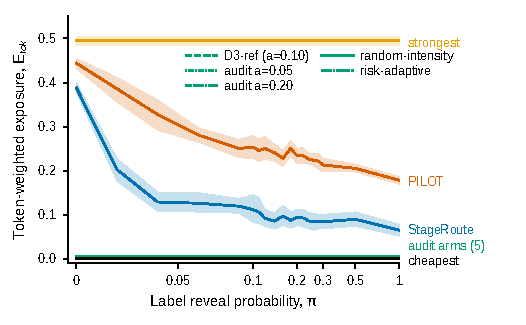
\includegraphics[width=\linewidth]{figures/figC_40seller_Etok_vs_pi.pdf}
  \caption{Billed-token-weighted $\Emet_{\mathrm{tok}}$ vs.\ $\pi$ at 40 sellers (secondary; primary $\Emet$ is per purchase). Lines are means over $n=20$ seeds; bands are 95\% paired-bootstrap CIs (10,000 resamples). The five audit arms share one colour and differ by line style. The $\pi$ axis is symmetric-log (linear below $\pi=0.08$).}
  \Description{Line chart of billed-token-weighted E against reveal probability pi, with the same method shapes as the primary E curve: PILOT and StageRoute rise as pi falls, cheapest stays at 0, strongest is flat near 0.50, and audit arms are flat near 0.}
  \label{fig:etok}
\end{figure}

\paragraph{$\pistar$ crossover (T2, 40 sellers).}
$\Delta J = J(\text{D3 reference}) - \max(J_{\text{StageRoute}}, J_{\text{PILOT}})$ with the best bandit taken per seed, paired over seeds (Table~\ref{tab:pistar}). Pre-registered rule: keep $(0.10,0.12)$ only if the interval at $\pi=0.12$ is entirely $<0$ and at $\pi=0.10$ entirely $>0$. $\Delta J$ is positive at every $\pi$, already $+0.114$ [$+0.104$, $+0.122$] at $\pi=1$, and all 20 seeds have no crossover (None: 20; non-monotone: 0). Therefore $(0.10,0.12)$ is \textbf{not kept}, and the paper reports this conditional range with the per-seed distribution. This is an appendix result and is not used in the body as a ranking of D3 against the bandits.

\begin{table}[h]
\caption{Paired $\Delta J$ at 40 sellers (mean [95\% CI]) and number of seeds with $\Delta J>0$.}
\label{tab:pistar}
\footnotesize
\setlength{\tabcolsep}{4pt}
\begin{tabular}{@{}rcc@{}}
\toprule
$\pi$ & $\Delta J$ [95\% CI] & Seeds $\Delta J>0$ (of 20) \\
\midrule
1 & $+0.114$ [$+0.104$, $+0.122$] & 20 \\
0.5 & $+0.136$ [$+0.126$, $+0.145$] & 20 \\
0.3 & $+0.143$ [$+0.133$, $+0.153$] & 20 \\
0.28 & $+0.145$ [$+0.133$, $+0.157$] & 20 \\
0.26 & $+0.151$ [$+0.139$, $+0.164$] & 20 \\
0.24 & $+0.153$ [$+0.140$, $+0.165$] & 20 \\
0.22 & $+0.160$ [$+0.147$, $+0.173$] & 20 \\
0.2 & $+0.162$ [$+0.149$, $+0.175$] & 20 \\
0.18 & $+0.166$ [$+0.154$, $+0.178$] & 20 \\
0.16 & $+0.164$ [$+0.152$, $+0.178$] & 20 \\
0.14 & $+0.160$ [$+0.148$, $+0.172$] & 20 \\
0.12 & $+0.172$ [$+0.157$, $+0.186$] & 20 \\
0.11 & $+0.168$ [$+0.149$, $+0.186$] & 20 \\
0.1 & $+0.164$ [$+0.145$, $+0.182$] & 20 \\
0.08 & $+0.178$ [$+0.158$, $+0.197$] & 20 \\
0.06 & $+0.206$ [$+0.193$, $+0.219$] & 20 \\
0.04 & $+0.210$ [$+0.183$, $+0.236$] & 20 \\
0.02 & $+0.283$ [$+0.254$, $+0.309$] & 20 \\
0 & $+0.288$ [$+0.276$, $+0.299$] & 20 \\
\bottomrule
\end{tabular}
\end{table}

\noindent\textit{First batch (v0.1 scale).} Under the same pre-registered rule, $(0.10,0.12)$ was also not kept: at $\pi=0.12$, $\Delta J=-0.0363$ [$-0.0623$, $-0.0135$] (entirely $<0$), but at $\pi=0.10$ it was $-0.0251$ [$-0.0438$, $-0.0067$] (not $>0$). Per-seed first crossovers ranged from $(0,0.05)$ to $(0.2,1)$, with only 2 of 20 in $(0.10,0.12)$ and 3 non-monotone seeds (3, 8, and 14). \vzeroonenote

\paragraph{Per-mode $q$ (40 sellers, selected $\pi$).}
Tables~\ref{tab:qmode}--\ref{tab:qmodeb} report $q_{\mathrm{swap}}$, $q_{\mathrm{theft}}$, and $q_{\mathrm{downgrade}}$ (unweighted mean over listed tail rounds). $^{\circ}$: $\Qmet$ not identifiable. Cheapest is $^{\circ}$ at every $\pi$ (0/20 tail-trade runs).

\begin{table*}[h]
\caption{Per-mode seller intent for PILOT and StageRoute, 40 sellers, 20 seeds (mean [95\% CI]).}
\label{tab:qmode}
\footnotesize
\setlength{\tabcolsep}{2.2pt}
\renewcommand{\arraystretch}{0.92}
\begin{tabular}{@{}rcccccc@{}}
\toprule
$\pi$ & $q_{\mathrm{swap}}$ PILOT & $q_{\mathrm{theft}}$ PILOT & $q_{\mathrm{down.}}$ PILOT & $q_{\mathrm{swap}}$ StageRoute & $q_{\mathrm{theft}}$ StageRoute & $q_{\mathrm{down.}}$ StageRoute \\
\midrule
1 & \cil{0.897}{0.839}{0.944} & \cil{0.943}{0.926}{0.960} & \cil{0.912}{0.868}{0.944} & \cil{0.503}{0.478}{0.527} & \cil{0.710}{0.648}{0.774} & \cil{0.614}{0.582}{0.644} \\
0.5 & \cil{0.942}{0.905}{0.966} & \cil{0.940}{0.929}{0.950} & \cil{0.927}{0.898}{0.953} & \cil{0.488}{0.454}{0.523} & \cil{0.771}{0.714}{0.828} & \cil{0.636}{0.612}{0.659} \\
0.3 & \cil{0.922}{0.874}{0.960} & \cil{0.941}{0.917}{0.959} & \cil{0.856}{0.800}{0.906} & \cil{0.478}{0.452}{0.503} & \cil{0.817}{0.766}{0.867} & \cil{0.642}{0.613}{0.668} \\
0.2 & \cil{0.883}{0.822}{0.937} & \cil{0.950}{0.937}{0.962} & \cil{0.870}{0.802}{0.927} & \cil{0.504}{0.468}{0.541} & \cil{0.841}{0.804}{0.877} & \cil{0.665}{0.634}{0.700} \\
0.12 & \cil{0.879}{0.803}{0.940} & \cil{0.929}{0.906}{0.949} & \cil{0.844}{0.801}{0.885} & \cil{0.495}{0.462}{0.528} & \cil{0.860}{0.812}{0.907} & \cil{0.623}{0.590}{0.656} \\
0.1 & \cil{0.905}{0.857}{0.944} & \cil{0.917}{0.882}{0.948} & \cil{0.864}{0.819}{0.905} & \cil{0.504}{0.466}{0.543} & \cil{0.885}{0.849}{0.919} & \cil{0.676}{0.638}{0.714} \\
0.08 & \cil{0.916}{0.887}{0.941} & \cil{0.952}{0.941}{0.963} & \cil{0.841}{0.791}{0.886} & \cil{0.491}{0.454}{0.528} & \cil{0.898}{0.863}{0.932} & \cil{0.688}{0.653}{0.717} \\
0.06 & \cil{0.906}{0.864}{0.943} & \cil{0.903}{0.853}{0.937} & \cil{0.865}{0.834}{0.897} & \cil{0.504}{0.466}{0.544} & \cil{0.910}{0.874}{0.943} & \cil{0.683}{0.644}{0.721} \\
0.02 & \cil{0.836}{0.783}{0.884} & \cil{0.777}{0.749}{0.800} & \cil{0.862}{0.824}{0.899} & \cil{0.475}{0.455}{0.495} & \cil{0.954}{0.933}{0.969} & \cil{0.720}{0.682}{0.757} \\
0 & \cil{0.776}{0.753}{0.798} & \cil{0.796}{0.769}{0.820} & \cil{0.801}{0.783}{0.819} & \cil{0.486}{0.457}{0.513} & \cil{0.944}{0.930}{0.958} & \cil{0.621}{0.581}{0.659} \\
\bottomrule
\end{tabular}
\end{table*}

\begin{table*}[h]
\caption{Per-mode seller intent for the D3 reference and cheapest, 40 sellers, 20 seeds (mean [95\% CI]). $^{\circ}$: not identifiable.}
\label{tab:qmodeb}
\footnotesize
\setlength{\tabcolsep}{2.2pt}
\renewcommand{\arraystretch}{0.92}
\begin{tabular}{@{}rcccccc@{}}
\toprule
$\pi$ & $q_{\mathrm{swap}}$ D3-ref & $q_{\mathrm{theft}}$ D3-ref & $q_{\mathrm{down.}}$ D3-ref & $q_{\mathrm{swap}}$ cheapest & $q_{\mathrm{theft}}$ cheapest & $q_{\mathrm{down.}}$ cheapest \\
\midrule
1 & \cil{0.601}{0.542}{0.653} & \cil{0.504}{0.476}{0.530} & \cil{0.510}{0.477}{0.546} & \cil{0.514}{0.490}{0.537}$^{\circ}$ & \cil{0.485}{0.461}{0.509}$^{\circ}$ & \cil{0.524}{0.504}{0.542}$^{\circ}$ \\
0.5 & \cil{0.601}{0.543}{0.654} & \cil{0.504}{0.476}{0.531} & \cil{0.510}{0.477}{0.547} & \cil{0.514}{0.490}{0.538}$^{\circ}$ & \cil{0.485}{0.461}{0.508}$^{\circ}$ & \cil{0.524}{0.504}{0.542}$^{\circ}$ \\
0.3 & \cil{0.601}{0.541}{0.653} & \cil{0.504}{0.476}{0.530} & \cil{0.510}{0.477}{0.547} & \cil{0.514}{0.490}{0.537}$^{\circ}$ & \cil{0.485}{0.461}{0.509}$^{\circ}$ & \cil{0.524}{0.505}{0.542}$^{\circ}$ \\
0.2 & \cil{0.601}{0.542}{0.653} & \cil{0.504}{0.477}{0.530} & \cil{0.510}{0.477}{0.548} & \cil{0.514}{0.490}{0.538}$^{\circ}$ & \cil{0.485}{0.462}{0.508}$^{\circ}$ & \cil{0.524}{0.504}{0.542}$^{\circ}$ \\
0.12 & \cil{0.601}{0.542}{0.652} & \cil{0.504}{0.477}{0.530} & \cil{0.510}{0.477}{0.547} & \cil{0.514}{0.490}{0.537}$^{\circ}$ & \cil{0.485}{0.462}{0.508}$^{\circ}$ & \cil{0.524}{0.504}{0.542}$^{\circ}$ \\
0.1 & \cil{0.601}{0.543}{0.653} & \cil{0.504}{0.477}{0.530} & \cil{0.510}{0.477}{0.547} & \cil{0.514}{0.490}{0.537}$^{\circ}$ & \cil{0.485}{0.462}{0.508}$^{\circ}$ & \cil{0.524}{0.504}{0.542}$^{\circ}$ \\
0.08 & \cil{0.601}{0.542}{0.653} & \cil{0.504}{0.476}{0.531} & \cil{0.510}{0.477}{0.547} & \cil{0.514}{0.490}{0.538}$^{\circ}$ & \cil{0.485}{0.462}{0.508}$^{\circ}$ & \cil{0.524}{0.504}{0.543}$^{\circ}$ \\
0.06 & \cil{0.601}{0.542}{0.653} & \cil{0.504}{0.477}{0.530} & \cil{0.510}{0.476}{0.547} & \cil{0.514}{0.490}{0.537}$^{\circ}$ & \cil{0.485}{0.462}{0.508}$^{\circ}$ & \cil{0.524}{0.504}{0.542}$^{\circ}$ \\
0.02 & \cil{0.601}{0.542}{0.654} & \cil{0.504}{0.476}{0.530} & \cil{0.510}{0.476}{0.548} & \cil{0.514}{0.490}{0.538}$^{\circ}$ & \cil{0.485}{0.461}{0.508}$^{\circ}$ & \cil{0.524}{0.504}{0.542}$^{\circ}$ \\
0 & \cil{0.601}{0.542}{0.653} & \cil{0.504}{0.477}{0.530} & \cil{0.510}{0.477}{0.547} & \cil{0.514}{0.490}{0.537}$^{\circ}$ & \cil{0.485}{0.462}{0.508}$^{\circ}$ & \cil{0.524}{0.504}{0.543}$^{\circ}$ \\
\bottomrule
\end{tabular}
\end{table*}

\paragraph{Q-gate checks (Hedge, first batch; EXP3, 40 sellers).}
The formal 40-seller gate is fictitious play and just passes as in \S\ref{sec:metrics}: Kendall $\tau_a=0.643$ (23 concordant, 5 discordant) at every $\pi$, just over 0.6; we do not call the order stable. As a robustness check at $\pi=1$ under egreedy, the main-table audit $\Qmet$ (0.52--0.54) is the unweighted mean over all 20 seeds, including the 7--8 runs with no tail-segment trade---the protocol definition, which does not require a sale. Restricting the mean to tail-trade runs changes the D3 reference only from 0.538 to 0.536 (other audit arms similarly); $\Qmet$ on no-tail runs is not concentrated at 0.5 (about 0.39--0.62). Dropping the five audit arms whose identifiability is only 12--13/20 leaves PILOT, StageRoute, and strongest, with Kendall $\tau_a=1.0$ at every $\pi$. This column is robustness only and does not change the pre-registered eight-method gate. A Hedge check on the first batch gives Kendall $\tau=1.0$ for the three-policy $\Qmet$ ordering at all 11 $\pi$. At that v0.1 scale the front can only be read along $\Emet$; StageRoute's $\Qmet$ is not identifiable, so no conclusion is drawn about front membership. With three policies, $\tau\ge0.6$ only means an identical order; Hedge does not count toward the gate. \vzeroonenote

The v1.0 48-round EXP3 check at the same 40-seller scale (20 seeds, compliance filter on, fixed roster) is appendix-only and does \emph{not} count toward the gate (Table~\ref{tab:exp3}). For all nine methods and all $\pi$, $\Qmet$ stays near 0.501 (intervals about [0.487, 0.515]), consistent with not learning in 48 rounds; no $\Qmet$ change vs.\ $\pi=1$ is significant. $\Emet$ still rises as $\pi$ falls: PILOT 0.110 [0.107, 0.114] at $\pi=1$, 0.134 [0.124, 0.145] at 0.10, and 0.220 [0.212, 0.229] at 0, with the increase vs.\ $\pi=1$ significant at every lower $\pi$; StageRoute 0.046 [0.038, 0.053] at $\pi=1$, 0.078 [0.066, 0.091] at 0.10, and 0.207 [0.198, 0.216] at 0, with the increase vs.\ $\pi=1$ significant at every $\pi\le 0.14$. Because sellers barely learned to attack, absolute $\Emet$ levels must not be compared with the egreedy main table.

\begin{table}[h]
\caption{EXP3 appendix (40 sellers, 20 seeds): $\Emet$ for the bandit routers at selected $\pi$ (mean [95\% CI]). $\Qmet$ is near 0.501 for every method and $\pi$ (see text). Not part of the Q-gate.}
\label{tab:exp3}
\footnotesize
\begin{tabular}{@{}rcc@{}}
\toprule
$\pi$ & $\Emet$ PILOT & $\Emet$ StageRoute \\
\midrule
1 & 0.110 [0.107, 0.114] & 0.046 [0.038, 0.053] \\
0.10 & 0.134 [0.124, 0.145] & 0.078 [0.066, 0.091] \\
0 & 0.220 [0.212, 0.229] & 0.207 [0.198, 0.216] \\
\bottomrule
\end{tabular}
\end{table}

\paragraph{Delist trade-off (T3).} Fixed-rate audit $a=0.1$, \code{reputation_rounds}$\in\{0,5,20\}$: $\Emet$, $\Qmet$ over listed rounds, suspended rounds, suspended-period $q$, \code{n_audits}: \TBD{T3-delist: table}. Longer delist can lower $\Emet$ while the learned $q$ including suspended rounds rises from missing observations; this is why $\Qmet$ excludes suspended rounds.

\paragraph{Adaptive audit under equal expected budget (T3).} Fixed vs.\ risk-adaptive at target $a=0.1$, escrow on: $\Emet$, $\Qmet$, \code{n_audits}, realized $a$, escrow held/slashed/released: \TBD{T3-adaptive: table}. Adaptive targeting is a cost/aiming comparison, not a claimed improvement.

\paragraph{T4 official setting (D3 reference, $\pi=1$).}
The official run uses \code{fixed_audit_a0.10}, $\pi=1$, seeds 0--19, and \code{--resample-roster} (Table~\ref{tab:t4counts}). Scores are on sellers who traded in the target window, not every seller on the roster. Train: 7 positives among 208 scored sellers (3 swap, 4 theft, 0 downgrade). Test: 2 positives among 89 scored sellers (1 swap, 1 theft); downgrade is skipped. Only 2 of 6 test runs have both classes for the \code{any} label (seeds 16 and 18, one positive each), which is below the reporting threshold of 4/6 definable runs. We therefore do not report detection performance and do not interpret the latency ablation. This sparsity matches the policy's rare trade with strategic sellers (this batch $\Emet=0.0066$). The post-5b simulator split remains \TBD{T4-5b}.

A calculation that pools the 89 test sellers across runs is \emph{not} the protocol (which requires a per-run score, then an average over runs) and is recorded only here: for \code{any} with logistic regression, pooled AUROC $=0.977$ and AP $=0.417$ on 89 sellers (2 positives); the 7-vs-6-feature $\Delta$AUROC is $+0.040$ $[0.011, 0.076]$. We do not read these figures as detection performance or as evidence about latency. Paths: \code{results/v1.0/t4_eval/} (original export, unchanged) and \code{results/v1.0/t4_eval_per_run/} (per-run recompute).

\begin{table}[h]
\caption{T4 official setting: D3 reference, $\pi=1$, resampled roster; features in rounds 1--32, labels in rounds 33--48. Counts are sellers who traded in the target window.}
\label{tab:t4counts}
\small
\setlength{\tabcolsep}{3pt}
\begin{tabular}{@{}lrrrrr@{}}
\toprule
Split & Scored & Any & Swap & Theft & Down. \\
\midrule
Train (0--13) & 208 & 7 & 3 & 4 & 0 \\
Test (14--19) & 89 & 2 & 1 & 1 & 0 \\
\bottomrule
\end{tabular}
\end{table}

\paragraph{T4 supplement (PILOT, $\pi=1$, current simulator).}
This run uses PILOT at $\pi=1$, the same train/test split, and a resampled roster, on the current simulator (before the 5b change). It does not replace the official D3 setting, which still does not report detection performance. All six test runs have both classes for \code{any} and for each attack type (Table~\ref{tab:t4pilotcounts}). Official metrics are the mean of per-test-run scores ($B=2000$; Table~\ref{tab:t4pilot}). This batch $\Emet=0.158$, with tail-segment trades in 20/20 runs. Under this setting only, the without-latency logistic AUROC $0.895$ exceeds the rule baseline $0.703$ in all six test runs; we do not claim that detection is equally strong without latency. Latency contributes on \code{any} (both models' $\Delta$AUROC intervals exclude 0), but the logistic-regression $\Delta$AUROC intervals for swap ($+0.065$ [$-0.019$, $+0.158$]) and downgrade ($+0.144$ [$-0.024$, $+0.301$]) contain 0. Downgrade is clearly weaker (logistic AUROC $0.826$, AP $0.458$, precision@10 $0.167$); theft is near ceiling (logistic AUROC $0.995$, AP $0.972$, precision@10 $0.300$). Path: \code{results/v1.0/t4_pilot_eval/}. Pooled-over-sellers figures in that export are not the protocol and are not reported here. The post-5b split remains \TBD{T4-5b}.

\begin{table}[h]
\caption{T4 supplement: PILOT, $\pi=1$, current simulator, resampled roster; features in rounds 1--32, labels in rounds 33--48. Counts are sellers who traded in the target window.}
\label{tab:t4pilotcounts}
\small
\setlength{\tabcolsep}{3pt}
\begin{tabular}{@{}lrrrrr@{}}
\toprule
Split & Scored & Any & Swap & Theft & Down. \\
\midrule
Train (0--13) & 524 & 105 & 40 & 34 & 31 \\
Test (14--19) & 215 & 49 & 18 & 18 & 13 \\
\bottomrule
\end{tabular}
\end{table}

\begin{table*}[h]
\caption{T4 supplement (PILOT, $\pi=1$, current simulator): official mean of per-test-run scores on the any-attack label ($B=2000$; all six test runs scored). The 7-feature column is the full whitelist; 6-feature drops latency. The rule baseline uses no latency, so the two columns coincide.}
\label{tab:t4pilot}
\small
\setlength{\tabcolsep}{8pt}
\begin{tabular}{@{}lcccc@{}}
\toprule
Model & AUROC 7 / 6 & $\Delta$AUROC & AP 7 / 6 & P@10 7 / 6 \\
\midrule
Logistic regression & $0.970$ [$0.941$, $0.991$] / $0.895$ & $+0.074$ [$0.039$, $0.108$] & $0.931$ / $0.772$ & $0.750$ / $0.583$ \\
GBDT & $0.976$ / $0.941$ & $+0.035$ [$0.017$, $0.051$] & $0.946$ / $0.859$ & $0.783$ / $0.650$ \\
Rule & $0.703$ / $0.703$ & $0$ & $0.493$ / $0.493$ & $0.400$ / $0.400$ \\
\bottomrule
\end{tabular}
\end{table*}

\clearpage
\paragraph{First batch (v0.1 scale) T2 table, figures, and reading.}
The following were the first v1.0 batch at v0.1 scale (3 sellers, one strategic seller using swap and theft only, 11-point $\pi$ grid) and are not the 40-seller main result.

\begin{table*}[h]
\caption{T2 first batch: $\Emet$ and $\Qmet$ vs.\ $\pi$ (mean [95\% CI], 20 seeds, $L=0$) and fraction of runs with tail-segment trades (StageRoute / PILOT / D3). $^{\circ}$: most runs have no tail trades, so $\Qmet$ is not identifiable (hollow points in the figures). $\Qmet$ is the simple mean of $q_{\mathrm{swap}}$ and $q_{\mathrm{theft}}$ ($q_{\mathrm{downgrade}}$ n/a at v0.1 scale). D3 reference values are constant in $\pi$ by construction. \vzeroonenote}
\label{tab:t2v01}
\footnotesize
\setlength{\tabcolsep}{3pt}
\begin{tabular}{@{}rccccccc@{}}
\toprule
$\pi$ & $\Emet$ StageRoute & $\Emet$ PILOT & $\Emet$ D3 ref. & $\Qmet$ StageRoute & $\Qmet$ PILOT & $\Qmet$ D3 ref. & Tail-trade runs \\
\midrule
1 & 0.014 [0.008, 0.020] & 0.046 [0.038, 0.054] & 0.106 [0.085, 0.131] & 0.689 [0.602, 0.783]$^{\circ}$ & 0.913 [0.860, 0.953] & 0.118 [0.061, 0.187] & 10\% / 75\% / 100\% \\
0.2 & 0.030 [0.014, 0.049] & 0.072 [0.063, 0.082] & 0.106 [0.085, 0.131] & 0.671 [0.584, 0.767]$^{\circ}$ & 0.912 [0.857, 0.951] & 0.118 [0.059, 0.187] & 0\% / 85\% / 100\% \\
0.18 & 0.026 [0.012, 0.044] & 0.090 [0.078, 0.102] & 0.106 [0.086, 0.130] & 0.698 [0.604, 0.795]$^{\circ}$ & 0.911 [0.854, 0.953] & 0.118 [0.060, 0.188] & 0\% / 95\% / 100\% \\
0.15 & 0.024 [0.012, 0.038] & 0.083 [0.069, 0.099] & 0.106 [0.086, 0.131] & 0.677 [0.592, 0.767]$^{\circ}$ & 0.929 [0.902, 0.954] & 0.118 [0.060, 0.189] & 10\% / 100\% / 100\% \\
0.12 & 0.036 [0.017, 0.061] & 0.087 [0.072, 0.102] & 0.106 [0.086, 0.131] & 0.746 [0.654, 0.839]$^{\circ}$ & 0.901 [0.839, 0.950] & 0.118 [0.060, 0.188] & 10\% / 85\% / 100\% \\
0.11 & 0.042 [0.022, 0.067] & 0.087 [0.073, 0.102] & 0.106 [0.085, 0.131] & 0.791 [0.696, 0.884]$^{\circ}$ & 0.881 [0.810, 0.941] & 0.118 [0.059, 0.187] & 5\% / 100\% / 100\% \\
0.1 & 0.047 [0.030, 0.066] & 0.092 [0.077, 0.106] & 0.106 [0.086, 0.131] & 0.822 [0.726, 0.910]$^{\circ}$ & 0.904 [0.851, 0.947] & 0.118 [0.059, 0.188] & 15\% / 95\% / 100\% \\
0.08 & 0.041 [0.024, 0.064] & 0.107 [0.089, 0.127] & 0.106 [0.086, 0.130] & 0.805 [0.709, 0.897]$^{\circ}$ & 0.914 [0.856, 0.954] & 0.118 [0.059, 0.188] & 10\% / 100\% / 100\% \\
0.06 & 0.053 [0.032, 0.077] & 0.118 [0.100, 0.135] & 0.106 [0.086, 0.130] & 0.840 [0.748, 0.923]$^{\circ}$ & 0.911 [0.861, 0.953] & 0.118 [0.059, 0.188] & 10\% / 95\% / 100\% \\
0.05 & 0.063 [0.035, 0.094] & 0.123 [0.103, 0.144] & 0.106 [0.085, 0.131] & 0.860 [0.775, 0.933]$^{\circ}$ & 0.904 [0.843, 0.951] & 0.118 [0.060, 0.187] & 10\% / 95\% / 100\% \\
0 & 0.083 [0.076, 0.089] & 0.684 [0.675, 0.694] & 0.106 [0.086, 0.130] & 0.934 [0.912, 0.955] & 0.937 [0.912, 0.960] & 0.118 [0.059, 0.188] & 100\% / 100\% / 100\% \\
\bottomrule
\end{tabular}
\end{table*}

\begin{figure*}[h]
  \centering
  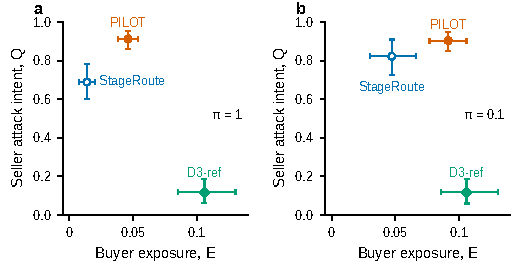
\includegraphics[width=0.5\textwidth]{figures/fig2_v01scale_pareto_EQ.pdf}
  \caption{First batch: $(\Emet,\Qmet)$ at $\pi=1$ (a) and $\pi=0.1$ (b). Points are means over $n=20$ seeds; bars are 95\% paired-bootstrap CIs (10,000 resamples). Hollow points: most runs have no tail-segment trades (StageRoute: 10\% and 15\% of runs), so $\Qmet$ is not identifiable. \vzeroonenote}
  \Description{Two scatter panels of buyer exposure E against seller intent Q for StageRoute, PILOT, and the D3 reference baseline at pi = 1 and pi = 0.1, with interval bars; StageRoute is drawn hollow.}
  \label{fig:paretov01}
\end{figure*}

\begin{figure*}[h]
  \centering
  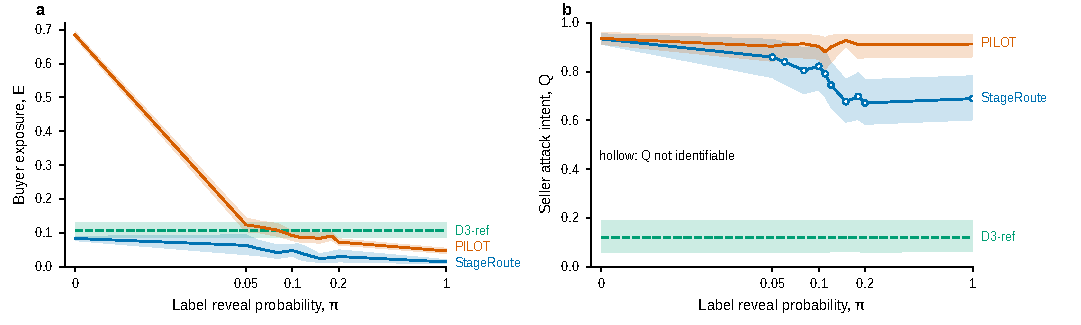
\includegraphics[width=\textwidth]{figures/fig3_v01scale_E_Q_vs_pi.pdf}
  \caption{First batch: buyer exposure $\Emet$ (a) and seller intent $\Qmet$ (b) vs.\ $\pi$ for StageRoute, PILOT, and the D3 reference (dashed; constant by construction). Lines are means over $n=20$ seeds; bands are 95\% paired-bootstrap CIs (10,000 resamples). Hollow points: StageRoute at every $\pi>0$. The $\pi$ axis is symmetric-log (linear below $\pi=0.05$). \vzeroonenote}
  \Description{Two line charts against reveal probability pi at v0.1 scale. Left: E for PILOT rises from about 0.05 at pi = 1 to about 0.68 at pi = 0; StageRoute rises from about 0.01 to about 0.08; D3 reference is flat near 0.11. Right: Q for PILOT stays near 0.9; StageRoute, drawn hollow for pi > 0, lies between about 0.67 and 0.93; D3 reference is flat near 0.12.}
  \label{fig:t2v01}
\end{figure*}

\paragraph{Reading (first batch, v0.1 scale only).} Bandits lower $\Emet$ by avoidance; when labels become sparse, avoidance fails and $\Emet$ rises. For sellers that are avoided and not trading, $\Qmet$ is not identifiable, and for those sellers this setting does not support conclusions about deterrence.
\begin{itemize}
\item \textbf{$\Emet$.} PILOT rises from 0.046 at $\pi=1$ to 0.123 at $\pi=0.05$ and 0.684 at $\pi=0$; StageRoute from 0.014 to 0.063 and 0.083. Against $\pi=1$ (paired, Holm over $\pi$), the increase is significant for PILOT at every $\pi\le0.2$ and for StageRoute at every $\pi\le0.12$.
\item \textbf{StageRoute $\Qmet$.} For $\pi>0$ only 0--15\% of StageRoute runs have tail trades, so its $\Qmet$ is not identifiable (hollow points). $\Qmet$ is statistically higher than at $\pi=1$ at $\pi=0.06$ and $0.05$ (Holm), but this comes from the $\sim$10\% of runs with tail trades and is not interpreted as a deterrence change. Its only identifiable point is $\pi=0$ (0.934), from which we do not generalize.
\item \textbf{PILOT $\Qmet$.} PILOT still buys from attackers (75--100\% of runs with tail trades), so $\Qmet$ is identifiable; it stays at 0.881--0.937 and shows no significant decrease at any $\pi$. Under this setting's seller learning rule and at v0.1 scale, PILOT does not lower seller attack intent.
\item \textbf{D3 reference.} $\Qmet=0.118$ and $\Emet=0.106$ at every $\pi$. Only their invariance in $\pi$ holds by construction (audits do not use labels); the values themselves depend on the audit rate and slashing parameters. D3's lower $\Qmet$ than PILOT's holds only under this setting's audit and slashing parameters ($a=0.1$) and the current seller learning rule. This is not evidence that audits deter attacks in general. D3 is a reference point for comparison, not a method.
\end{itemize}
T2 in this batch uses \code{reputation_rounds=0}: no suspension occurs and no rounds are excluded from $\Qmet$.

\section{Protocol clarifications after the first batch}
\label{app:amend}
The protocol was frozen before the 40-seller main table was run. After the first (v0.1-scale) batch, two definitions that the protocol left ambiguous were clarified and recorded in \code{docs/PROTOCOL_v1.0.md}; reading rules and thresholds were not changed.
\begin{enumerate}
\item \textbf{$\Qmet$ is unweighted.} $\Qmet$ is the unweighted mean of $q$ over the rounds in which the seller is present (listed, not suspended); the primary column is the simple average across attack types ($q_{\mathrm{swap}}$, $q_{\mathrm{theft}}$, $q_{\mathrm{downgrade}}$). The earlier token weighting is undefined when a seller has no trades in the tail segment.
\item \textbf{$\Emet$ denominator is purchases.} $\Emet=$ attacked served purchases / served purchases, matching the simulator's metrics code. The billed-token-weighted $\Emet_{\mathrm{tok}}$ is a secondary side column.
\end{enumerate}

\section{RQ coverage}
\label{app:rq}

This appendix maps nearby research questions onto the v1.0 pack. It \textbf{does not} expand the paper's claims.

\begin{table*}[h]
\caption{RQ coverage (v1.0 vs later).}
\label{tab:rq}
\footnotesize
\setlength{\tabcolsep}{3pt}
\begin{tabularx}{\textwidth}{@{}>{\raggedright\arraybackslash}p{2.3cm} >{\raggedright\arraybackslash}X >{\raggedright\arraybackslash}p{2.4cm} >{\raggedright\arraybackslash}p{2.5cm} >{\raggedright\arraybackslash}p{2.9cm} >{\raggedright\arraybackslash}p{3.2cm}@{}}
\toprule
RQ & Example task & Inputs & Labels / supervision & Metrics & Coverage \\
\midrule
\textbf{T1--T3 (protocol)} & Fixed-rate deterrence; sparse-label degradation; equal-budget adaptive (appendix) & \code{episodes} (+\code{orders}/\code{audits}) & episode eval only & $\Emet$, $\Qmet$ (primary, gated); \code{n_audits} for T3 & \textbf{v1.0} \\
\textbf{T4 seller risk ranking} & Rank sellers by future fraud & 7 whitelisted features & held-out fraud labels (rounds 33--48) & AUROC, AP, P@10 & \textbf{v1.0} (two simulator versions) \\
\textbf{A2 multi-jurisdiction compliance} & Hard-filter violation / route reachability; filter-off control & \code{buyers}+\code{orders}(+\code{sellers}) & path $\times$ \code{compliance_profile} (derived) & violation rate, fill rate & \textbf{v1.0 basic} --- not a full regulatory rule library \\
\textbf{A1 provenance (weak)} & Order $\rightarrow$ claimed/actual model $\rightarrow$ audit trail & \code{orders}$\bowtie$\code{audits}$\bowtie$\code{sellers} & \code{actual_model} (label) & trail completeness; weak ID accuracy & \textbf{v1.0 weak} --- trade/audit trail only \\
\textbf{A1 provenance (strong)} & Content-level provenance chain & needs hashes + parent links & content/output match & provenance-chain accuracy & \textbf{later} \\
\textbf{C1 market mechanism} & Posted-price + audit-rate protocols & \code{orders}+\code{episodes}+\code{audits} & episode eval & $\Emet$, $\Qmet$, volume, \code{n_audits} & \textbf{v1.0 partial} (posted-price only; \textbf{no auction}) \\
\textbf{C1 auctions} & Bid / clear / allocate & needs mechanism fields & allocation labels & efficiency, revenue & \textbf{later} \\
\textbf{Resale / rewrite / distill} & Downstream reuse of upstream inference & needs event layer & \code{source_order_id}, \code{downstream_model_id} & provenance-chain match & \textbf{later} \\
\bottomrule
\end{tabularx}
\end{table*}

%% =====================================================================
%% Draft "References" key->title map (human-readable; refs.bib is authoritative):
%%   becker1968crime, avenhaus2002inspection, daughety2008communicating,
%%   bester2001strategic, bester2021signaling, hanson2003combinatorial,
%%   wolfers2004prediction, uma2024optimistic, polymarket2024resolution,
%%   panda2025pilot, li2026stageroute, iosco2009surveillance,
%%   cumming2008surveillance, cumming2019capital, aws2024compute_sla
%% v1.0 text edits 2026-11-10 (Asia/Shanghai): see CHANGES_v1.0.md.
\end{document}
